% ============================================================
% Procedural Generation of Attention: Gaze Trajectories and
% the Grammar of Cinematic Space
% Flyxion — Independent Researcher
% ============================================================

\documentclass[12pt, a4paper]{article}

\usepackage{fontspec}
\setmainfont{TeX Gyre Pagella}

\usepackage{amsmath, amssymb, amsthm}
\usepackage{mathtools}
\usepackage{geometry}
\geometry{margin=1.25in}

\usepackage{setspace}
\setstretch{1.4}

\usepackage{hyperref}
\hypersetup{
  colorlinks=true,
  linkcolor=black,
  citecolor=black,
  urlcolor=black
}

\usepackage{booktabs}
\usepackage{enumitem}
\usepackage{tikz}
\usetikzlibrary{arrows.meta, positioning}

% ------------------------------------------------------------
% Theorem environments
% ------------------------------------------------------------
\theoremstyle{plain}
\newtheorem{theorem}{Theorem}[section]
\newtheorem{proposition}[theorem]{Proposition}
\newtheorem{lemma}[theorem]{Lemma}
\newtheorem{corollary}[theorem]{Corollary}

\theoremstyle{definition}
\newtheorem{definition}[theorem]{Definition}
\newtheorem{example}[theorem]{Example}

\theoremstyle{remark}
\newtheorem{remark}[theorem]{Remark}

% ------------------------------------------------------------
% Custom commands
% ------------------------------------------------------------
\newcommand{\X}{\mathcal{X}}
\newcommand{\A}{\mathcal{A}}
\newcommand{\G}{\mathcal{G}}
\newcommand{\N}{\mathcal{N}}
\newcommand{\Traj}{\Gamma}
\newcommand{\traj}{\gamma}
\newcommand{\AG}{A_G}
\newcommand{\salience}{w}
\newcommand{\reward}{R}
\newcommand{\jerk}{J}

% ------------------------------------------------------------

\title{%
  Procedural Generation of Attention:\\
  Gaze Trajectories and the Grammar of Cinematic Space%
}
\author{Flyxion\\[4pt]
  \small Independent Researcher}
\date{}

\begin{document}

\maketitle

% ------------------------------------------------------------
\begin{abstract}
We propose a formal theory of \emph{admissibility-guided
traversal} and use cinema as its primary motivating example.
The central claim is that designed systems generate
experience by shaping admissibility structures $(\X, \A)$
that constrain and guide trajectories through possibility
spaces. A designer constructs $(\X, \A)$; an observer
generates a trajectory $\traj$ satisfying $\traj(t+1) \in
\A(\traj(t))$; experience emerges from the properties of
$\traj$ rather than from the terminal state $\traj(T)$
alone. This structure --- which we call a \emph{traversal
system} --- is instantiated by cinema, game design, musical
composition, and mathematical proofs, among other systems.

In cinema, the state space is the visual fixation field
$\G_t$, and $\A$ is determined by salience gradients,
saccadic transport cost, and editing structure. We show that
the gaze density field evolves according to a
Fokker--Planck advection-diffusion equation driven by the
salience function, that camera movement induces a
vector-field coupling whose stability is governed by the
smooth pursuit threshold, and that classical editing
conventions --- the 180-degree rule, eyeline matching, the
30-degree rule --- emerge as approximate solutions to a
re-acquisition minimization over gaze anchor density,
derivable from perceptual principles without reference to
narrative convention.

We then establish the \emph{Traversal Reward
Decomposition}: $\reward(\traj) = \reward(\traj(T)) +
\reward_T(\traj)$, where $\reward_T$ is a traversal reward
that is non-zero for non-degenerate admissibility structures
and independent of informational novelty. This explains why
replay, rewatching, rereading, rehearsal, and ritual are not
anomalous. Wim Wenders' \textit{Perfect Days} is examined
as a natural experiment in which $\reward_T \gg
\reward(\traj(T))$, isolating traversal reward from terminal
reward. The \emph{Traversal Equivalence} theorem shows that
cinema, games, music, and proofs are structurally identical
at the level of $(\X, \A, \traj)$; the film--game
correspondence table follows as a corollary rather than an
analogy. The \emph{Designer--Observer Separation} theorem
formalizes the bilateral structure of designed experience:
the designer controls $\A$; the observer generates $\traj$;
neither fully determines experience unilaterally. The
framework generates empirical predictions testable by
eye-tracking and psychophysiological methods and points
toward a general account of admissibility-structured
cognition that extends from perceptual attention through
play, ritual, and education.
\end{abstract}

\tableofcontents
\newpage

% ============================================================
\section{Introduction}
\label{sec:intro}
% ============================================================

Film theory traditionally begins with narrative. Attention
research begins with fixation. Game studies begins with
interaction. This paper begins with traversal.

The three fields have each generated substantial knowledge
about designed experience. Film theory has illuminated how
stories are structured, how meaning is constructed across
shots, and how editing produces coherence from discontinuity.
Attention research has documented how the eye moves through
visual fields, what salience factors drive fixation, and how
perceptual systems extract information from scenes. Game
studies has developed accounts of interactivity, player
agency, and the design of navigable spaces. What none of
these traditions has done is identify the common substrate
that underlies all three.

That substrate is traversal. We propose that cinema, game
design, music, and other forms of designed experience are
all instances of the same formal structure: a designer
constructs an admissibility structure $(\X, \A)$ over a
state space, and an observer generates a trajectory $\traj$
through that structure satisfying $\traj(t+1) \in
\A(\traj(t))$. Experience emerges from properties of the
trajectory rather than from the terminal state alone. The
designer does not control the observer's path. The designer
controls what paths are possible.

\begin{equation}
  (\X, \A) \;\longrightarrow\; \traj
  \;\longrightarrow\; \reward(\traj)
  \label{eq:traversal_diagram}
\end{equation}

\begin{figure}[h]
\centering
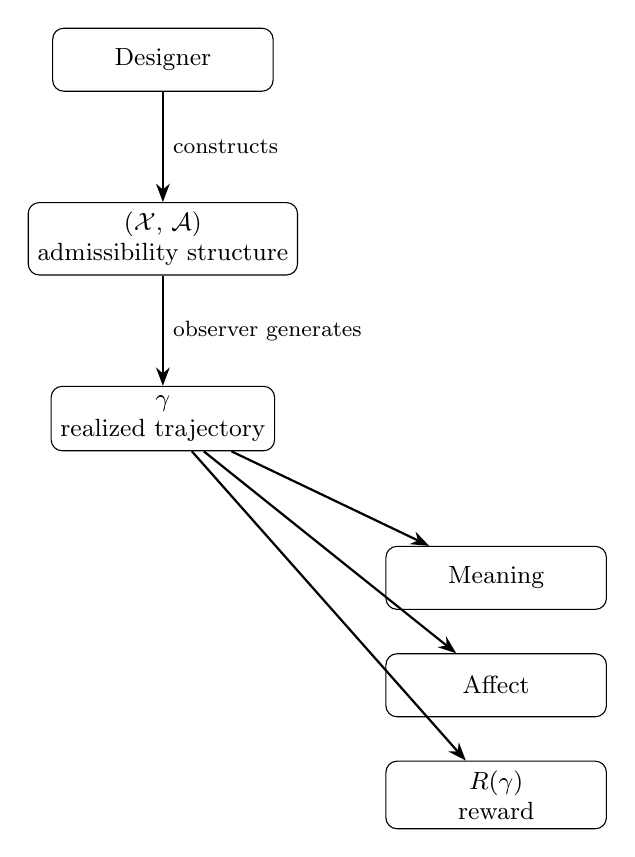
\begin{tikzpicture}[
  node distance=1.4cm and 2.6cm,
  box/.style={draw, rounded corners, minimum width=2.8cm,
    minimum height=0.8cm, align=center, font=\small},
  arr/.style={-{Stealth}, thick}
]
  \node[box] (designer) {Designer};
  \node[box, below=of designer] (xa) {$(\X,\,\A)$\\admissibility structure};
  \node[box, below=of xa] (traj) {$\traj$\\realized trajectory};
  \node[box, below right=1.2cm and 1.4cm of traj] (meaning) {Meaning};
  \node[box, below=0.55cm of meaning] (affect) {Affect};
  \node[box, below=0.55cm of affect] (reward) {$\reward(\traj)$\\reward};

  \draw[arr] (designer) -- node[right, font=\footnotesize]
    {constructs} (xa);
  \draw[arr] (xa) -- node[right, font=\footnotesize]
    {observer generates} (traj);
  \draw[arr] (traj) -- (meaning);
  \draw[arr] (traj) -- (affect);
  \draw[arr] (traj) -- (reward);
\end{tikzpicture}
\caption{The organizing structure of the traversal
  framework. The designer constructs $(\X, \A)$; the
  observer generates $\traj$ by local admissible steps;
  meaning, affect, and reward emerge as properties of
  $\traj$ rather than of the terminal state $\traj(T)$.}
\label{fig:traversal_diagram}
\end{figure}

Diagram~\eqref{eq:traversal_diagram} is the organizing
structure of the paper. The left arrow is the designer's
contribution: specifying a state space and a transition
function. The middle arrow is the observer's contribution:
generating a trajectory by local admissible steps. The right
arrow is experience: the reward, affect, and meaning that
emerge from properties of the trajectory rather than from
its endpoint.

We begin with gaze because it is measurable. Eye-tracking
technology makes gaze trajectories directly observable,
and the extensive literature on visual attention provides
a solid empirical foundation for the spatial claims of
Sections~\ref{sec:spatial} and~\ref{sec:trajectory}. But
gaze is the entry point, not the subject. The framework
developed here applies equally to locomotion through a game
level, expectation through a musical phrase, and inference
through a mathematical proof. The proof case is the
strongest demonstration that the theory is genuinely about
traversal: when the same formal structure that describes
gaze control in cinema also describes the experience of
reading a known proof, the framework has reached something
more general than vision.

The paper proceeds as follows. Section~\ref{sec:spatial}
introduces the screen as a weighted fixation field and
describes cinematic devices as geometric operations on that
field. Section~\ref{sec:trajectory} develops the theory of
gaze trajectories, formalizes the cut as a discontinuity
event, derives editing grammar from a re-acquisition
minimization, and states the procedural generation claim
precisely. Section~\ref{sec:kinetic} distinguishes spatial
from temporal guidance and shows that camera movement,
editing rhythm, object motion, and musical phrasing are all
operations on the same temporal geometry. Section~\ref{sec:affect}
shows how the spatial and temporal structures of the
preceding sections give rise to recurring affective
operations, without proposing a general theory of emotion.
Section~\ref{sec:empirical} states the framework's empirical
predictions. Section~\ref{sec:unified} steps back to show
that film, games, music, and proofs are all traversal
systems in the sense of the formal definition, locates prior
research traditions within the framework, and argues that
traversal is intrinsically rewarding independent of
informational novelty. Section~\ref{sec:conclusion} returns
to the traversal claim as a demonstrated result.

% ============================================================
\section{The Screen as Spatial Field}
\label{sec:spatial}
% ============================================================

\subsection{The Frame as a Weighted Fixation Field}
\label{subsec:frame}

A frame contains objects. This is how films are ordinarily
described: a room, two characters, a gun on the table. But
this description operates at the wrong level for the present
analysis. Before the viewer identifies any object, before
narrative content is assigned to anything on screen, the
frame has already done something more primitive: it has
defined a distribution over possible fixation points. The
filmmaker's first task is not to tell a story but to shape
the topology of the fixation field.

\begin{definition}[Gaze Field]
  At time $t$, the \emph{gaze field} is a pair
  $(\G_t, \salience_t)$ where $\G_t = \{g_1, g_2, \ldots,
  g_n\}$ is the set of candidate fixation points in the
  current frame and $\salience_t : \G_t \to [0,1]$ is a
  salience function assigning to each point a weight
  proportional to the probability that an unconstrained
  viewer will fixate it. Salience is determined jointly by
  motion, luminance contrast, edge density, face presence,
  implied gaze vectors, text, and color singularity.
\end{definition}

The salience function $\salience_t$ is not uniform. In any
given frame, some regions attract fixation far more strongly
than others. A face in a scene of ambient background will
draw the eye with near-universal consistency across viewers.
A moving object in an otherwise static frame will capture
attention before its identity is recognized. These are not
aesthetic preferences but perceptual facts about the human
visual system, extensively documented in eye-tracking
research \cite{yarbus1967,itti1998}.

What follows from this is that every compositional decision
--- where to place actors, where to direct light, what
aperture to use, how to set the camera height --- is a
decision about $(\G_t, \salience_t)$. The composition is
not primarily a picture. It is a distribution. Two frames
containing identical narrative content but different
compositions produce different distributions, direct the
eye differently, and produce different experiences even
when a viewer could describe both in the same words.

We can quantify the degree of attention control a given
frame achieves by measuring the entropy of its salience
distribution.

\begin{definition}[Salience Entropy]
  The \emph{salience entropy} of a frame at time $t$ is
  \begin{equation}
    S(\G_t)
    = -\sum_{g_i \in \G_t}
      \salience_t(g_i) \log \salience_t(g_i).
  \end{equation}
  $S(\G_t)$ is maximized when $\salience_t$ is uniform
  over $\G_t$ and minimized when $\salience_t$ concentrates
  all mass on a single fixation point.
\end{definition}

\begin{proposition}[Salience Concentration]
\label{prop:salience_concentration}
  Rack focus, localized illumination, and foreground
  isolation each decrease $S(\G_t)$. Consequently these
  operations reduce the effective number of admissible
  fixation targets.
\end{proposition}

\begin{proof}
  Each operation transfers probability mass from a broad
  distribution over $\G_t$ to a concentrated distribution
  over a proper subset $\G'_t \subsetneq \G_t$. Since
  entropy is maximized by the uniform distribution and
  strictly decreases under mass concentration,
  $S(\G'_t) < S(\G_t)$. The effective fixation set
  --- the number of candidates with non-negligible
  salience weight --- contracts accordingly.
\end{proof}

Proposition~\ref{prop:salience_concentration} makes precise
what it means to say that a rack focus or key light
``controls'' viewer attention. Control is not binary. It
is a continuous reduction in $S(\G_t)$, measurable in
principle from the salience distribution induced by any
given composition. A perfectly controlled frame has
$S(\G_t) \approx 0$; a completely uncontrolled frame has
$S(\G_t) = \log |\G_t|$. Most film compositions operate
in the middle of this range, with deliberate moments of
high control (a face in a spotlight) and deliberate moments
of low control (an establishing wide shot inviting
exploration).

The salience function is not merely a static weighting. In
any continuous shot it changes over time as objects move,
light shifts, and the camera reframes. To capture this
dynamics we model gaze density as a field evolving under
salience.

\begin{definition}[Gaze Density Field]
  The \emph{gaze density field} $\rho(g, t)$ is a
  probability density over $\G_t$ representing the
  distribution of fixations across a population of viewers
  at time $t$, normalized so that
  $\int_{\G_t} \rho(g,t)\, dg = 1$.
\end{definition}

\begin{theorem}[Salience Flow]
\label{thm:salience_flow}
  Let $\salience_t : \G_t \to [0,1]$ be continuously
  differentiable in both $g$ and $t$. Then the gaze density
  field $\rho(g,t)$ evolves according to the
  advection-diffusion equation
  \begin{equation}
    \frac{\partial \rho}{\partial t}
    = -\nabla \cdot \bigl(\rho\, \nabla \salience_t\bigr)
      + D\,\Delta\rho,
    \label{eq:salience_flow}
  \end{equation}
  where $D \geq 0$ is an exploration parameter governing
  the rate of diffusion of gaze away from salience peaks.
  Consequently, regions of high salience act as attractors
  of fixation density: in the limit $D \to 0$, $\rho$
  concentrates on the maxima of $\salience_t$.
\end{theorem}

\begin{proof}
  Model each viewer's fixation as a particle moving in the
  salience landscape under gradient ascent perturbed by
  Brownian noise: $d\traj = \nabla \salience_t\, dt +
  \sqrt{2D}\, dW_t$. The Fokker--Planck equation for the
  density of such particles is exactly
  \eqref{eq:salience_flow}. In the zero-noise limit
  $D \to 0$ the diffusion term vanishes and the flow is
  pure gradient ascent, concentrating mass on salience
  maxima.
\end{proof}

Theorem~\ref{thm:salience_flow} connects the static
analysis of Section~\ref{subsec:frame} to the dynamic
trajectory analysis of Section~\ref{sec:trajectory}. The
filmmaker who reshapes $\salience_t$ over time --- through
movement within the frame, lighting changes, or camera
motion --- is modifying the vector field $\nabla
\salience_t$ that drives $\rho$. This is not merely
influencing where viewers look. It is specifying a
dynamical system whose attractors are the filmmaker's
intended fixation targets.

\subsection{Cinematic Devices as Geometric Operations}
\label{subsec:devices}

The tools available to a cinematographer can be understood
as a set of operations on the gaze field $(\G_t,
\salience_t)$. Describing them in these terms clarifies
what they do at the perceptual level, prior to any
interpretation of their narrative function.

\medskip
\noindent\textbf{Rack focus.} A rack focus shifts the lens
focal plane from one depth to another within the frame,
throwing the previously sharp region into blur and bringing
the newly focused region into clarity. In gaze field terms,
this is a salience annihilation operation:

\begin{equation}
  \salience_t(g_i) \to 0 \quad \text{for all } g_i
  \text{ outside the new focal plane}
\end{equation}

The number of candidate fixation points in $\G_t$ does not
change. The number of high-salience fixation points collapses
to the focused region. The filmmaker does not tell the viewer
where to look. The filmmaker destroys the salience of every
alternative.

\medskip
\noindent\textbf{Lighting.} A lighting setup shapes the
salience field across the entire frame by controlling the
distribution of luminance contrast. Hard directional light
creates steep salience gradients, concentrating the
distribution around bright regions and deep shadows. Flat
ambient light produces a shallow gradient and a diffuse
distribution. When a key light isolates a face in an
otherwise dark frame, it performs salience concentration by
luminance means rather than optical means. The effect on
$\salience_t$ is structurally identical to a rack focus:
the viewer's eye is given little alternative to the lit
region.

\medskip
\noindent\textbf{Blocking.} The placement of actors within
the frame distributes high-salience objects --- faces,
bodies in motion, implied gaze vectors --- across $\G_t$.
A scene in which two actors stand at opposite edges of a
wide frame creates a split distribution with two competing
attractors and a low-salience region between them. A scene
in which one actor stands close to camera while another
recedes into background creates a depth hierarchy in
$\salience_t$. The director blocking a scene is engineering
this distribution: determining which regions of the frame
will compete for the viewer's attention and in what order.

\medskip
\noindent\textbf{Framing and focal length.} The choice of
lens and camera distance determines how much spatial world
is projected onto the frame, how much background competes
with foreground for salience, and how much of $\G_t$ is
occupied by the primary subject. A long lens compresses
depth, reduces background detail, and concentrates
$\salience_t$ on the subject. A wide lens expands the
field, increases the number of candidate fixation points,
and widens the distribution.

\subsection{The Game Level as Analogous Spatial Field}
\label{subsec:gamelevel}

A game level is a navigable volume rather than a projected
frame, but it operates on the player's gaze field by
identical means. The level designer controls a spatial
environment from which the player's visual attention must be
directed toward intended targets, guided through intended
paths, and managed across an extended traversal.

The toolkit is structurally the same. Lighting in a game
environment concentrates salience exactly as lighting on a
film set does: a bright opening at the end of a dark
corridor draws the player's eye and locomotion toward it
precisely as a key light draws the viewer's gaze to a face.
Architectural funneling --- the use of converging walls,
narrowing passages, and forced perspectives --- constrains
$\G_t$ spatially, reducing candidate fixation directions and
biasing the player toward the intended path. A highlighted
interactable object, marked by a glow, a distinctive color,
or an animation, is a salience concentration operation
identical to a rack focus: the designer destroys the
relative salience of the surrounding environment to force
attention to the target.

The differences between a film frame and a game level are
real but secondary from this perspective. A frame is a
two-dimensional projection; a level is a three-dimensional
volume. A film viewer cannot redirect the camera; a player
can redirect their gaze within the available volume. But in
both cases the designer's task is the same: construct a
salience field $(\G_t, \salience_t)$ that channels attention
toward intended regions while leaving the observer the
subjective experience of choosing where to look. Effective
spatial design in both film and games produces the experience
of free attention while delivering constrained attention.
The observer feels they are looking where they choose.
They are looking where the designer arranged.

% ============================================================
\section{Trajectory Generation}
\label{sec:trajectory}
% ============================================================

\subsection{Gaze Trajectories}
\label{subsec:gazetraj}

The gaze field $(\G_t, \salience_t)$ defined in
Section~\ref{subsec:frame} specifies where the eye
\emph{could} go at any moment. It does not specify where
the eye \emph{will} go. Between these two questions lies
the theory of gaze trajectories: the study of how the
perceptual system generates a path through the fixation
field rather than merely responding to individual frames.

\begin{definition}[Gaze Trajectory]
  A \emph{gaze trajectory} is a path $\traj : [0,T] \to \G$
  through fixation space, where $\G = \bigcup_t \G_t$ is
  the total fixation space across all frames. At each
  moment $t$, the trajectory specifies the current fixation
  $\traj(t) \in \G_t$. The set of locally admissible
  continuations from $\traj(t)$ is denoted $\Traj(\traj(t))$.
\end{definition}

The critical property of gaze trajectories is that they are
not arbitrary paths through $\G$. The eye does not sample
the fixation field randomly. At each moment, the next
fixation is generated from the current fixation by a
process that is simultaneously bottom-up (driven by the
salience field) and top-down (constrained by task, history,
and expectation). This dual determination is the source of
the filmmaker's leverage: by controlling $\salience_t$, the
filmmaker shapes the bottom-up component of trajectory
generation even when the top-down component varies across
viewers.

\begin{proposition}[Local Trajectory Constraint]
\label{prop:local_constraint}
  Let $\traj(t)$ denote the current fixation. Then the
  probability distribution over the next fixation
  $\traj(t+1)$ is jointly determined by:
  \begin{enumerate}[label=\emph{(\roman*)}]
    \item local salience gradients $\nabla \salience_t$
      in the neighborhood of $\traj(t)$,
    \item saccadic transport cost $d(\traj(t), g_i)$
      for each candidate $g_i \in \G_t$,
    \item task constraints specifying which regions are
      task-relevant at time $t$, and
    \item prior fixation history $\traj(0), \ldots,
      \traj(t-1)$, encoding inhibition of return and
      scene memory.
  \end{enumerate}
  Consequently, gaze trajectories are locally constrained
  traversals of $\G$, not arbitrary paths. The admissibility
  structure $\A$ governing trajectory generation is
  determined by factors (i)--(iv) jointly.
\end{proposition}

Proposition~\ref{prop:local_constraint} has an important
corollary for the theory of cinematic control. The
filmmaker directly controls factor (i) through
cinematography and composition. Factors (ii) is a fixed
property of the oculomotor system. Factor (iii) is shaped
partly by the filmmaker through narrative cues that
establish task relevance. Factor (iv) is a function of the
film's prior shots and therefore also under the filmmaker's
indirect control. This means the filmmaker has leverage
over three of the four determinants of the next fixation.
The impression that the viewer is freely directing their
own gaze is accurate at the phenomenological level and
misleading at the mechanistic level.

Two consequences follow for the structure of the paper.
First, the transition from gaze fields to gaze trajectories
is not a change of subject but a deepening of the same
analysis: the field specifies the distribution at a moment,
the trajectory specifies how that distribution is traversed
over time. Second, the four-factor structure of
Proposition~\ref{prop:local_constraint} implies that
trajectory generation is a genuinely local process ---
each fixation is determined by the current state and
immediate neighborhood, not by global knowledge of the
film --- which is precisely the condition under which
procedural generation in the sense of Section~\ref{subsec:procedural}
is the right description of what is happening.

The local character of trajectory generation also implies
a structural fact about gaze paths that motivates the
special status of cuts.

\begin{proposition}[Piecewise Continuity]
\label{prop:piecewise_continuity}
  For sufficiently small temporal intervals $\Delta t$
  between saccadic events,
  \begin{equation}
    d\bigl(\traj(t + \Delta t),\, \traj(t)\bigr)
    < \varepsilon
  \end{equation}
  for some $\varepsilon$ bounded by oculomotor constraints.
  Consequently, gaze trajectories are piecewise continuous
  paths through $\G$, with discontinuities occurring only
  at saccadic events.
\end{proposition}

\begin{proof}
  Between saccades, the eye is in fixation: its angular
  position changes by at most the drift rate of the
  oculomotor system, which is small relative to the scale
  of the fixation field. The bound $\varepsilon$ is
  therefore determined by physiology rather than by the
  film. Discontinuities in $\traj$ occur only when a
  saccade is initiated, which is a discrete event with
  non-zero inter-saccade intervals.
\end{proof}

Proposition~\ref{prop:piecewise_continuity} is the formal
grounding for why cuts are special. Within a continuous
shot, gaze trajectories are continuous: the eye traverses
$\G_t$ smoothly, guided by the salience field and the
camera motion field $V_t$. A cut introduces a discontinuity
in $\G_t$ itself, not merely in $\traj$: the frame changes
instantaneously. The perceptual system must then generate
a new fixation from a standing start, which is the
re-acquisition problem formalized in
Section~\ref{subsec:cut}. Camera movements that are
continuous in $\G_t$ are therefore qualitatively different
from cuts, not merely faster or slower versions of the
same event.

The local selection of the next fixation point can be
stated as an explicit optimization.

\begin{proposition}[Least-Effort Saccade Principle]
\label{prop:least_effort}
  The expected next fixation satisfies
  \begin{equation}
    \traj(t+1)
    = \arg\max_{g_i \in \G_t}
      \Bigl(
        \salience_t(g_i)
        - \lambda\, d\bigl(\traj(t), g_i\bigr)
      \Bigr),
    \label{eq:least_effort}
  \end{equation}
  where $\lambda > 0$ is a cost coefficient weighting
  saccadic transport distance against informational gain.
  Fixation selection therefore balances the pull of salience
  against the cost of movement.
\end{proposition}

\begin{proof}[Proof sketch]
  Equation~\eqref{eq:least_effort} follows from treating
  the oculomotor system as approximately optimizing an
  immediate expected utility: the benefit of fixating $g_i$
  is proportional to the information potentially gained,
  which is captured by $\salience_t(g_i)$, and the cost
  is the metabolic and temporal cost of the saccade,
  which is proportional to angular distance $d(\traj(t),
  g_i)$. Under a linear utility model the optimizer takes
  the stated form. This is consistent with empirical models
  of saccadic selection \cite{itti1998} and with the
  inhibition-of-return phenomenon, which reduces
  $\salience_t(g_i)$ for recently visited locations.
\end{proof}

Proposition~\ref{prop:least_effort} has a direct
consequence for cinematography. The filmmaker who places a
high-salience target near the current expected fixation
position imposes lower transport cost and therefore higher
probability of rapid acquisition. Placing a high-salience
target at the far edge of the frame simultaneously raises
the salience term and the cost term in
\eqref{eq:least_effort}. Whether the target is acquired
depends on the ratio $\salience_t(g_i) / (\lambda\,
d(\traj(t), g_i))$. The filmmaker managing this ratio
across a scene is implicitly solving the same optimization
that the viewer's oculomotor system is solving locally.

\subsection{Camera Movement as Trajectory Imposition}
\label{subsec:camera}

Camera movement acts on the gaze trajectory by introducing
a systematic, time-varying displacement of the entire
fixation field. Where the operations of Section~\ref{subsec:devices}
modified the salience distribution within a static frame,
camera movement modifies the frame itself: it translates,
rotates, scales, or perturbs $\G_t$ as a whole, imposing
a motion on every candidate fixation point simultaneously.

We formalize this as a vector field on the gaze space.

\begin{definition}[Camera Motion Field]
  At time $t$, a camera movement induces a \emph{camera
  motion field} $V_t : \G_t \to T\G_t$, assigning to each
  candidate fixation point $g_i \in \G_t$ a displacement
  vector $V_t(g_i)$ in the tangent space of $\G_t$. The
  induced trajectory displacement is
  $\traj(t+dt) = \traj(t) + V_t(\traj(t)) \cdot dt$
  in the limit of continuous camera motion.
\end{definition}

Each camera move corresponds to a characteristic class of
vector field on $\G_t$.

\medskip
\noindent\textbf{Pan.} A horizontal pan translates the
entire gaze field laterally at a uniform rate. The field
$V_t$ is approximately constant across $\G_t$: every
fixation point is displaced by the same vector. The pan
carries the eye along a constrained horizontal path
regardless of which fixation point within the field it
currently occupies. This is trajectory imposition in the
clearest sense: the viewer can resist the pan by fixating
against its direction, but the salience field is also
moving, so resistance requires active effort and produces
the experience of looking away from what the film wants
to show.

\medskip
\noindent\textbf{Dolly and tracking.} A dolly or tracking
shot moves the camera through physical space, producing a
parallax displacement that varies with depth: nearby
objects appear to move rapidly across the field while
distant objects move slowly. The field $V_t$ is therefore
non-uniform, with magnitude increasing as a function of
proximity. The viewer experiences this as locomotion:
the visual system interprets depth-dependent parallax as
self-motion through a stable environment. This is why the
dolly and the zoom, which produce superficially similar
screen effects, feel phenomenologically different. The
dolly provides the full parallax signature of locomotion
and triggers the proprioceptive correlates of movement.
The zoom does not.

\medskip
\noindent\textbf{Zoom.} A zoom changes focal length without
moving the camera, scaling the entire image toward or away
from its center. The induced field $V_t$ is a radial
expansion or contraction centered on the frame center:
$V_t(g_i) \propto (g_i - c)$ where $c$ is the center
point. The zoom produces the visual appearance of approach
or retreat without the parallax signature of actual
locomotion. The perceptual system receives conflicting
information: the image says approach, the vestibular system
says stationary. The characteristic affective quality of
the zoom --- unease, dream-like dislocation, the sense of
something wrong with the movement --- follows directly from
this conflict between the optical and proprioceptive
channels. The dolly and zoom are not stylistic variants.
They are geometrically distinct operations producing
different sensorimotor signatures.

\medskip
\noindent\textbf{Handheld.} A handheld camera introduces
stochastic perturbation into $V_t$: the field is no longer
smooth but noisy, with high-frequency random displacements
overlaid on any intentional camera movement. In trajectory
terms, this widens the locally admissible fixation set at
each moment: the viewer cannot predict exactly where a
given region of interest will be in the next instant. The
uncertainty is not merely informational. It is perceptual:
the visual system must continuously re-acquire its target
as the field perturbs around it. The physical correlate of
handheld imagery --- bodily instability, urgency,
documentary authenticity --- arises because the perturbation
pattern matches the signature of a moving, unstable
observer rather than a fixed camera platform.

\medskip
The camera motion field $V_t$ is the filmmaker's most
direct instrument for trajectory imposition because it
acts on the gaze trajectory independently of where within
the frame the viewer happens to be looking. Salience shapes
the distribution over $\G_t$; $V_t$ moves $\G_t$ itself.
The two instruments operate at different levels of the
trajectory generation process and can be combined or
opposed to produce complex effects: a pan that moves the
salience field in one direction while a bright object
appears at the frame edge in the opposite direction
creates a competition between $V_t$ and $\salience_t$,
and the tension of that competition is experienced directly
by the viewer as a pull between two attentional demands.

The relationship between $V_t$ and the resulting gaze
trajectory can be stated as a formal alignment claim.

\begin{proposition}[Trajectory Alignment]
\label{prop:trajectory_alignment}
  Let $V_t : \G_t \to T\G_t$ be a coherent motion field
  induced by camera movement. Then expected gaze velocity
  aligns with $V_t$ up to bounded error:
  \begin{equation}
    \mathbb{E}\bigl[\dot{\traj}(t)\bigr]
    = \alpha V_t(\traj(t)) + \epsilon_t
  \end{equation}
  where $\alpha > 0$ is a coupling coefficient determined
  by the relative strength of camera motion against
  competing salience signals, and $\epsilon_t$ is a
  zero-mean error term bounded by oculomotor noise and
  task-driven deviations.
\end{proposition}

\begin{proof}[Proof sketch]
  A coherent camera motion field displaces every candidate
  fixation point in $\G_t$ by $V_t(g_i) \cdot dt$ in
  a small interval $dt$. If the viewer is currently
  fixating $\traj(t)$, the target of the fixation moves
  to $\traj(t) + V_t(\traj(t)) \cdot dt$. The smooth
  pursuit system of the oculomotor apparatus tracks moving
  targets at velocities up to approximately
  $30^\circ\,\text{s}^{-1}$; within this range, gaze
  velocity matches target velocity with high fidelity.
  The coupling coefficient $\alpha$ falls below unity when
  camera speed exceeds the smooth pursuit limit, inducing
  corrective saccades. The error term $\epsilon_t$
  accumulates competing salience signals that may redirect
  gaze against the camera motion.
\end{proof}

Proposition~\ref{prop:trajectory_alignment} formally
states what pans and tracking shots accomplish: they induce
a coherent $V_t$ that the oculomotor system tracks,
carrying the gaze trajectory with the camera within the
bounds of the smooth pursuit system. The dolly, pan, tilt,
and tracking shot are all instances of coherent $V_t$
fields with different geometric structures; the handheld
camera is a stochastic $V_t$ that disrupts alignment and
forces increased $\epsilon_t$.

When camera speed remains below the smooth pursuit
threshold, gaze does not merely align with camera
motion on average — it locks onto the moving target
asymptotically.

\begin{theorem}[Tracking Stability]
\label{thm:tracking_stability}
  Suppose $\|V_t\| < V_c$ for all $t$, where $V_c$ is
  the smooth-pursuit velocity threshold of the oculomotor
  system. Let $g^\ast(t)$ denote the intended target
  position moving under $V_t$. Then
  \begin{equation}
    \lim_{t \to \infty}
    \bigl\| \traj(t) - g^\ast(t) \bigr\| = 0.
  \end{equation}
  That is, sufficiently smooth camera motion induces
  asymptotically stable gaze locking onto the moving
  target.
\end{theorem}

\begin{proof}
  Under the smooth pursuit system, the oculomotor error
  $e(t) = \traj(t) - g^\ast(t)$ evolves according to a
  first-order error-correction loop: $\dot{e} = -k e +
  \eta(t)$ where $k > 0$ is the pursuit gain and $\eta(t)$
  is bounded noise. When $\|V_t\| < V_c$, the pursuit
  system does not saturate and maintains $k > 0$. The
  homogeneous solution $e(t) = e(0)e^{-kt}$ decays to
  zero, and the forced response due to $\eta$ remains
  bounded. Hence $e(t) \to 0$ as $t \to \infty$.
\end{proof}

Theorem~\ref{thm:tracking_stability} provides the
mathematical explanation for why slow tracking shots feel
effortless while fast pans feel effortful. Below $V_c$
the smooth pursuit system maintains a stable lock and the
viewer experiences the camera's motion as natural
continuation. Above $V_c$ the pursuit system saturates,
corrective saccades become necessary, and the eye
repeatedly loses and re-acquires the target — the
perceptual correlate of a pan that feels too fast to
follow.

\subsection{The Cut as Discontinuity Event}
\label{subsec:cut}

Every cut is a discontinuity in the gaze trajectory. Where
camera movement carries the eye along a continuous path
through the fixation field, the cut resets the field
instantaneously: the frame before the cut is replaced by a
frame that may share none of its spatial structure. The
viewer's perceptual system must locate a new fixation target
from a standing start.

Formally, let $\traj(t^-)$ denote the gaze position
immediately before a cut and $\traj(t^+)$ the gaze position
immediately after. The cut introduces a discontinuity
$\traj(t^-) \neq \traj(t^+)$ in general, and the
perceptual system faces what we call the \emph{re-acquisition
problem}: given the new frame $F_{t+1}$ and the prior
fixation $\traj(t^-)$, find the intended target in $F_{t+1}$
as rapidly as possible.

\begin{definition}[Re-acquisition Cost]
  The re-acquisition cost $C(F_t, F_{t+1})$ of a cut from
  frame $F_t$ to frame $F_{t+1}$ is the time and attentional
  effort required for the viewer's gaze to reach the
  filmmaker's intended target region in $F_{t+1}$, given
  the fixation state $\traj(t^-)$ at the moment of the cut.
\end{definition}

Re-acquisition cost is not uniform across cuts. It depends on
the relationship between the two frames. Specifically, it
depends on the degree to which structures present in $F_t$
survive into $F_{t+1}$ in a form that can guide the eye
toward its new target. We formalize this as the gaze anchor
relation.

\begin{definition}[Gaze Anchor Relation]
  The gaze anchor relation $\AG(F_t, F_{t+1})$ is the set
  of perceptual structures that persist across consecutive
  frames $F_t, F_{t+1}$, grounding the inference that a
  common world underlies both and providing guidance for
  post-cut fixation. Anchor structures include: screen
  position, motion vector, luminance peak, face location,
  and implied gaze direction.
\end{definition}

When $|\AG(F_t, F_{t+1})|$ is large, the viewer's eye has
multiple guides into the new frame and re-acquisition is
rapid. When $|\AG|$ is small, the eye must search the new
frame with little guidance, re-acquisition is slow, and the
cut may register as disorienting or jarring. A jump cut ---
a cut between two shots of the same subject from nearly the
same angle --- is disorienting not because it violates
narrative expectations but because it destroys spatial
anchor density while preserving just enough similarity that
the viewer cannot determine whether a cut has occurred at
all. An incoherent edit --- a cut between entirely unrelated
spaces with no shared structure --- destroys anchor density
entirely, producing confusion.

The relationship between anchor density and re-acquisition
cost can be stated precisely.

\begin{theorem}[Anchor Bound]
\label{thm:anchor_bound}
  There exists a monotone decreasing function
  $f : \mathbb{N} \to \mathbb{R}^+$ such that
  \begin{equation}
    C(F_t, F_{t+1}) \leq f\bigl(|\AG(F_t, F_{t+1})|\bigr).
  \end{equation}
  Consequently, increasing anchor density provides an
  upper bound on re-acquisition cost: more anchors
  guarantee faster target acquisition after a cut.
\end{theorem}

\begin{proof}
  Each anchor structure $a \in \AG(F_t, F_{t+1})$
  provides an independent cue that the perceptual system
  can use to locate the intended target in $F_{t+1}$.
  With $|\AG| = 0$, no cues are available and acquisition
  reduces to visual search over the entire frame, with
  cost bounded below by mean search time. With
  $|\AG| = k > 0$, at least one of $k$ independent cues
  points toward the target region; the expected time to
  locate the target decreases with $k$ since the observer
  need only follow any one cue successfully. Define
  $f(k) = C_{\max} \cdot \prod_{i=1}^{k}(1 - p_i)^{-1}$
  where $p_i$ is the probability that the $i$-th anchor
  type successfully guides acquisition and $C_{\max}$ is
  the cost of uninstructed search; then $f$ is monotone
  decreasing in $k$ and provides the required bound.
\end{proof}

The Anchor Bound gives a monotone relationship between
anchor count and re-acquisition cost. We can sharpen this
into an information-theoretic statement by measuring the
quality of anchors, not merely their number.

\begin{definition}[Anchor Entropy]
\label{def:anchor_entropy}
  The \emph{anchor entropy} of a cut from $F_t$ to
  $F_{t+1}$ is
  \begin{equation}
    H_A(F_t, F_{t+1})
    = -\sum_{i} p_i \log p_i,
  \end{equation}
  where $p_i$ is the probability that anchor $i \in
  \AG(F_t, F_{t+1})$ successfully predicts the location
  of the intended target in $F_{t+1}$. Low anchor entropy
  means one or a few anchors predict the target with high
  reliability; high anchor entropy means all anchors are
  uncertain.
\end{definition}

\begin{theorem}[Information-Theoretic Cut Cost]
\label{thm:cut_entropy}
  Re-acquisition cost satisfies
  \begin{equation}
    C(F_t, F_{t+1}) \propto H_A(F_t, F_{t+1})
  \end{equation}
  up to perceptual constants. Cuts with low anchor entropy
  have low re-acquisition cost; cuts with high anchor
  entropy are costly regardless of the number of anchors
  present.
\end{theorem}

\begin{proof}
  Model target acquisition after a cut as an optimal
  search problem. With anchor predictions $\{p_i\}$, the
  minimum expected search cost is achieved by testing
  anchors in decreasing order of $p_i$. The expected number
  of tests before success is $\sum_i i \cdot p_i (1 -
  p_1)\cdots(1-p_{i-1})$, which is a monotone increasing
  function of $H_A$ when the $p_i$ are permuted toward
  uniformity. In the limit of uniform $p_i$ (maximum
  entropy), all anchors are equally unreliable and expected
  search cost reaches its maximum; in the limit of a single
  $p_i = 1$ (zero entropy), the target is located
  immediately. The proportionality to $H_A$ holds to first
  order in the entropy expansion of the search cost.
\end{proof}

Theorem~\ref{thm:cut_entropy} refines the Anchor Bound by
distinguishing cuts that have many anchors but uncertain
ones from cuts with few anchors that are individually
reliable. An eyeline match is a low-entropy cut: the gaze
direction anchor predicts the target location with high
probability. A cut to a wide shot of an unfamiliar
environment may have many candidate anchors, none
individually reliable, producing high $H_A$ and therefore
high re-acquisition cost despite the anchor count being
non-zero.
\label{subsec:grammar}

The grammar of continuity editing --- the accumulated
practical conventions by which professional editors join
shots --- can be understood as a set of heuristics for
maintaining high anchor density across cuts. We argue that
these conventions are not historically contingent stylistic
norms. They are approximate solutions to a perceptual
optimization problem. The closest antecedent in the
existing literature is the attentional theory of cinematic
continuity \cite{smith2012}, which argues that editing
conventions function primarily to guide and maintain viewer
attention. The present framework formalizes that claim:
anchor density is the quantity being maximized, and the
editing rules emerge as solutions to the resulting
optimization.

The optimization is:

\begin{equation}
  \min_{F_{t+1}} C(F_t, F_{t+1})
  \quad \text{subject to narrative constraint}
  \label{eq:reacquisition_min}
\end{equation}

That is: among the shots that could follow the current shot
given narrative requirements, choose the one that minimizes
re-acquisition cost. Equivalently, maximize $|\AG(F_t,
F_{t+1})|$.

The three most fundamental rules of continuity editing
emerge directly from this optimization.

\medskip
\noindent\textbf{The 180-degree rule.} In a scene involving
two characters in conversation, the camera must remain on one
side of an imaginary line connecting them. Crossing the line
reverses the apparent screen direction of each character,
destroying the motion-vector anchors established in prior
shots. A character who was moving left-to-right now appears
to move right-to-left without any corresponding narrative
event. The 180-degree rule is the solution to: preserve
motion-vector anchor structures across cuts involving
character movement. It persists not because editors were
taught it but because violations measurably increase
re-acquisition cost and produce viewer confusion.

\medskip
\noindent\textbf{Eyeline matching.} When a character looks
off-screen in one shot, the following shot should show the
object of their gaze from approximately the character's point
of view. The eyeline match preserves two anchor types
simultaneously: gaze direction (the character's look
establishes a vector that the next shot satisfies) and, often,
face location (the face appearing in shot B occupies the
region that the look in shot A pointed toward). Violations
produce the experience of a character looking at something
other than what the edit implies they see, again because the
anchor structure is broken.

\medskip
\noindent\textbf{The 30-degree rule.} Two consecutive shots
of the same subject should differ by at least 30 degrees of
camera angle. Violations produce the jump cut: the subject
appears to lurch forward in the frame because the screen
position anchor is too similar to signal that a cut has
occurred, yet different enough that spatial continuity is
disrupted. The 30-degree minimum is an approximate threshold
below which position anchors mislead rather than guide.

\begin{proposition}
\label{prop:grammar_as_optimization}
  The three primary rules of continuity editing are
  solutions to the re-acquisition minimization
  \eqref{eq:reacquisition_min} under the following
  correspondences: the 180-degree rule maximizes
  motion-vector anchor density; eyeline matching maximizes
  gaze-direction and face-position anchor density; the
  30-degree rule prevents the degenerate case in which
  position anchor similarity is high enough to suppress
  cut detection but low enough to disrupt spatial continuity.
\end{proposition}

\begin{corollary}[Grammar Emergence]
\label{cor:grammar_emergence}
  Any editing system trained solely to minimize
  re-acquisition cost $C(F_t, F_{t+1})$ across a corpus
  of cuts will converge toward the heuristics of
  continuity editing grammar, without access to narrative
  content or historically transmitted conventions.
\end{corollary}

\begin{proof}
  By Theorem~\ref{thm:anchor_bound}, minimizing $C$ is
  equivalent to maximizing $|\AG|$. By
  Proposition~\ref{prop:grammar_as_optimization}, the
  editing rules that maximize anchor density under the
  relevant geometric constraints are precisely the
  180-degree rule, eyeline matching, and the 30-degree
  rule. An optimizer of $C$ therefore converges to these
  rules as a consequence of the anchor bound alone.
\end{proof}

Corollary~\ref{cor:grammar_emergence} converts the
empirical claim about editing grammar into a theorem-derived
consequence. Film grammar is not a historical accident
encoding the aesthetic preferences of early Hollywood
editors. It is the approximately optimal solution to a
perceptual minimization problem. The prediction is that a
computational system with no knowledge of film history,
given only a model of human post-cut fixation behavior,
should rediscover these conventions.

\subsection{Game Locomotion as Explicit Trajectory Generation}
\label{subsec:gamelocomotion}

In cinema, the viewer's trajectory through the gaze field is
generated implicitly: the eye responds to salience signals
and anchor structures that the filmmaker has engineered, but
the eye's movement is not experienced as authored. In game
design, trajectory generation is made explicit: the player
moves through a navigable volume, and the experience of
movement is foregrounded rather than concealed.

Despite this difference in phenomenology, the underlying
structure is identical. The level designer constructs an
admissibility structure $(\X, \A)$ over a spatial volume:
$\X$ is the set of positions the player can occupy, and
$\A(x)$ specifies where the player can move from position
$x$ given the geometry of walls, floors, doors, and other
constraints. The player generates a trajectory $\traj$
satisfying $\traj(t+1) \in \A(\traj(t))$. The designer does
not control the player's path. The designer controls what
paths are possible.

The toolkit by which level designers shape $(\X, \A)$ maps
directly onto the filmmaker's toolkit for shaping $\G_t$.
Corridors are forced perspectives: they concentrate the
admissible trajectory set to a narrow band, exactly as a
rack focus concentrates the gaze field. Landmarks serve as
navigation markers: they are high-salience points that
attract the player's trajectory, exactly as a lighting cue
attracts the viewer's eye. Architectural funneling --- the
use of converging geometry to draw the player toward a
specific location --- is the spatial equivalent of the
camera pan, which carries the eye along a predetermined path.

This correspondence suggests that level design and
cinematography are the same discipline applied to different
observer modalities. The filmmaker engineers gaze; the level
designer engineers locomotion. Both are constructing
traversal systems.

\subsection{Procedural Generation of Attention}
\label{subsec:procedural}

The preceding sections have established that the filmmaker
shapes the gaze field $\G_t$, manages trajectory
admissibility through camera movement, and controls
re-acquisition cost through editing. It might appear from
this description that the filmmaker controls the viewer's
attention. This appearance is mistaken, and the mistake
matters.

The filmmaker does not determine where the viewer looks. The
filmmaker constructs an admissibility structure $(\X, \A)$
from which the viewer's trajectory emerges. The trajectory
is generated by the viewer, not by the film.

The gaze field $\G_t$ introduced in
Section~\ref{subsec:frame} is a specific realization of
this abstract structure: $\G_t \subseteq \X$, where $\X$ is
the full space of possible fixation states across the film.
At each moment $t$, the current frame exposes a subset of
$\X$ with a salience weighting $\salience_t$ over that
subset. The admissibility function $\A$ then specifies which
transitions among fixation states are locally reachable,
determined jointly by salience gradients, saccadic transport
cost, and camera motion as formalized in
Propositions~\ref{prop:local_constraint}
and~\ref{prop:least_effort}. The cinematic sections of the
paper are therefore a detailed instantiation of the general
traversal framework in the specific state space of visual
attention. The generalization to games, music, and proofs
in Section~\ref{sec:unified} consists of replacing $\G_t$
with the appropriate domain-specific state space while
leaving the structure $(\X, \A, \traj)$ unchanged.

\begin{equation}
  \traj(t+1) \in \A(\traj(t))
  \label{eq:trajectory_generation}
\end{equation}

The filmmaker specifies $\A$. The viewer generates $\traj$.
This is procedural generation in the strict sense of the
term: a system of local rules from which global structure
emerges through a generative process that the rule-specifier
does not directly control.

The analogy with game design is precise here. A game designer
does not control player movement. The designer constructs
walls, corridors, lighting gradients, and landmark
placements --- the local admissibility constraints --- and
the player's path emerges from their interaction with those
constraints. Two players in the same level generate
different trajectories. Two viewers of the same film generate
different gaze paths. In both cases, the designed structure
constrains but does not determine the observer's trajectory.

This framing resolves an apparent tension in film theory
between the claim that films exert powerful control over
viewer experience and the observation that viewers respond
differently to the same film. Both claims are correct. The
admissibility structure $(\X, \A)$ strongly constrains the
space of possible trajectories while leaving the specific
trajectory underdetermined. High-salience events, clear
anchor structures, and strong kinetic signals narrow $\A$
considerably, producing near-universal gaze behavior. Low
salience, weak anchors, and ambiguous kinetics widen $\A$,
producing divergent viewer trajectories. The filmmaker
manages the breadth of $\A$; the viewer traverses it.

The connection to ecological perception is worth noting
here. Gibson's affordances \cite{gibson1979} are the
action possibilities that an environment offers an
organism --- what it can do from a given position. In the
present framework, $\A(x)$ is precisely the set of
admissible continuations from state $x$: the afforded
trajectories. The filmmaker engineering $(\X, \A)$ is
constructing an environment of affordances for the viewer's
attention. Level designers have long operated with this
intuition implicitly; the traversal framework makes it
explicit and connects it to the formal theory of admissibility
structures.

% ============================================================
\section{Kinetic Synchronization}
\label{sec:kinetic}
% ============================================================

\subsection{Spatial and Temporal Guidance Distinguished}
\label{subsec:spatiotemporal}

Sections~\ref{sec:spatial} and~\ref{sec:trajectory} have
addressed a spatial question: given a frame, where can
attention go? The gaze field $\G_t$, the salience function
$\salience$, and the anchor relation $\AG$ all concern the
distribution of possible fixations across the two-dimensional
plane of the screen.

But guiding attention through space is only half the
filmmaker's task. There is a second, orthogonal dimension of
control: the temporal structure of when attention should
move, how rapidly transitions should occur, and what rhythm
of change the viewer's perceptual system should be entrained
to follow. This temporal dimension is the subject of the
present section, and it is here that the connection between
cinema, music, and game design becomes most explicit.

The key observation is that temporal guidance is a separable
system from spatial guidance. Music provides the clearest
demonstration. A musical phrase has no screen position. It
specifies no fixation point, creates no gaze anchor, and
shapes no salience field. Yet it powerfully organizes
temporal expectation: the listener anticipates the next
beat, the resolution of a dissonance, the return of a
theme. Music is pure temporal guidance operating without any
spatial component. This makes it a useful limiting case. By
examining what music and cinema share despite their obvious
differences, we can isolate the temporal guidance system
that cinema deploys alongside its spatial system.

\begin{definition}[Trajectory Rate of Change]
  Let $\Traj(t)$ denote the admissibility structure at time
  $t$. The trajectory rate of change is:
  \begin{equation}
    \Lambda(t) = \left| \frac{d\Traj}{dt} \right|
  \end{equation}
  measuring how rapidly the set of admissible continuations
  is being restructured. High $\Lambda(t)$ corresponds to
  rapid perceptual change; low $\Lambda(t)$ corresponds to
  stasis or slow development.
\end{definition}

Both a musical crescendo and a camera dolly increase
$\Lambda(t)$. Both a sustained note and a long static take
hold $\Lambda(t)$ near zero. The claim of this section is
that these are equivalent operations in different
representational media: both shape the temporal geometry of
the observer's trajectory through the admissibility
structure.

\begin{proposition}[Rhythmic Equivalence]
\label{prop:rhythmic_equivalence}
  Let $(\X_1, \A_1)$ and $(\X_2, \A_2)$ be traversal
  systems in different modalities with respective
  admissibility-rate profiles $\Lambda_1(t)$ and
  $\Lambda_2(t)$. If
  \begin{equation}
    \Lambda_1(t) = \Lambda_2(t) \quad \text{for all } t,
  \end{equation}
  then the two systems generate equivalent temporal guidance
  structures, independently of modality. Any observer
  traversing either system experiences the same temporal
  shape of constraint change.
\end{proposition}

\begin{proof}
  Temporal guidance is defined entirely in terms of
  $\Lambda(t)$: the rate at which the admissibility
  structure is being deformed. Two systems with identical
  $\Lambda(t)$ profiles impose identical rates of
  structural change on any observer trajectory, regardless
  of whether the underlying state space is visual,
  auditory, spatial, or logical. The modality determines
  the substrate of $\X$ and the sensory channel through
  which $\A$ is communicated to the observer; it does not
  enter the definition of $\Lambda(t)$.
\end{proof}

Proposition~\ref{prop:rhythmic_equivalence} licenses the
cross-modal claims of this section. A slow camera dolly
and a musical crescendo do not merely feel similar. When
their $\Lambda(t)$ profiles match, they are formally
equivalent temporal guidance operations. This is what
allows a film score to substitute for, reinforce, or
contradict the temporal guidance provided by the image
track: the two systems are operating on the same quantity.

The degree of alignment between image and music can be
quantified as an energy functional.

\begin{definition}[Synchronization Energy]
\label{def:sync_energy}
  Let $\Lambda_I(t)$ and $\Lambda_M(t)$ denote the
  admissibility-rate profiles of the image and music
  tracks respectively. The \emph{synchronization energy}
  is
  \begin{equation}
    E_{\mathrm{sync}}
    = \int_0^T
      \bigl(\Lambda_I(t) - \Lambda_M(t)\bigr)^2\, dt.
  \end{equation}
  $E_{\mathrm{sync}} = 0$ corresponds to perfect
  synchronization; large $E_{\mathrm{sync}}$ corresponds
  to strong desynchronization.
\end{definition}

\begin{proposition}[Resonance Principle]
\label{prop:resonance}
  Perceived kinetic synchronization between image and music
  is maximized when $E_{\mathrm{sync}} \to 0$, and
  perceived tension between the two tracks is monotone
  increasing in $E_{\mathrm{sync}}$. Synchronization and
  desynchronization are therefore a single variational
  parameter available to the filmmaker.
\end{proposition}

\begin{proof}
  By Proposition~\ref{prop:rhythmic_equivalence}, two
  tracks with identical $\Lambda(t)$ profiles generate
  equivalent temporal guidance. When image and music
  coincide ($E_{\mathrm{sync}} = 0$) the two guidance
  systems are aligned and reinforce each other with no
  perceptual tension between them. When they differ, the
  observer's temporal expectation system receives
  conflicting inputs from two channels; the conflict
  magnitude grows monotonically with the pointwise
  divergence $|\Lambda_I(t) - \Lambda_M(t)|$, and the
  integrated conflict is $E_{\mathrm{sync}}$.
\end{proof}

The Resonance Principle converts the filmmaker's
choice of music-to-image synchronization into a
variational problem: minimize $E_{\mathrm{sync}}$ for
reinforcement; maximize it for tension, irony, or
dissociation. The expressively neutral choice is not zero
synchronization energy but the energy that best serves
the moment's intended affective geometry.

\subsection{The Cut as Beat}
\label{subsec:cutbeat}

The cut is not only a spatial discontinuity event, as
analyzed in Section~\ref{subsec:cut}. It is also a temporal
event: a discrete pulse in the flow of the film. When cuts
occur at regular intervals, they establish a meter. When cut
frequency increases, tempo accelerates. When cuts cluster and
thin out, they produce rhythmic phrasing.

This is not metaphorical. Editing rhythm has measurable
effects on arousal and attentional engagement that are
independent of the semantic content of the shots being
joined. An action sequence cut at high frequency produces
physiological arousal not because the images depict
dangerous events but because rapid perceptual
discontinuities --- rapid spikes in $\Lambda(t)$ --- prime
the nervous system for response. The same images cut slowly
produce a different physiological state. The rhythm is
operating on the body before the content reaches
interpretation.

The equivalence with music is structural. A sequence of cuts
at regular intervals is a sequence of temporal events with a
defined period, exactly like a musical pulse. Irregular cuts
produce syncopation. A sudden acceleration of cut rate is a
rhythmic intensification. A cut held back past its expected
moment produces the same effect as a delayed beat: tension
sustained by withholding the anticipated event.

\subsection{Camera Movement as Phrase}
\label{subsec:phrase}

Where cuts produce discrete temporal events, camera
movements produce continuous temporal shapes. A camera move
has onset, duration, and resolution, exactly as a musical
phrase does. The structural parallels are close enough to
warrant explicit mapping.

A slow push-in toward a subject develops over time, building
gradually, and resolves when the camera reaches its endpoint
or cuts away. This is the temporal shape of a sustained tone
moving toward a crescendo: continuous increase in $\Lambda(t)$
culminating in a release. The emotional correlate --- a
growing sense of attention, of approach, of something about
to be revealed --- is a product of this temporal shape, not
of the content being approached.

A whip pan is a percussive accent: a brief, violent spike in
$\Lambda(t)$ followed by immediate return to a new stable
state. It marks a moment without developing it, exactly as a
cymbal crash marks a rhythmic position without sustaining a
melody.

A long take with a static or slowly moving camera holds
$\Lambda(t)$ near zero for an extended period. This is the
temporal equivalent of a sustained note or a fermata: a
deliberate withholding of change that produces tension
through its very stillness. The viewer's anticipation of
future change accumulates during the hold, so that when
motion or a cut finally arrives, its effect is amplified
by the stored expectation.

\subsection{Object Movement as Kinetic Event}
\label{subsec:objectmovement}

Camera movement is not the only source of temporal structure
within a shot. Objects moving within the frame produce
kinetic events that are rhythmic before they are semantic.
An actor crossing from one side of the frame to the other
has a duration, a pace, and a moment of arrival. A vehicle
accelerating through the frame has an onset and a peak. A
door closing is a brief event with a definite endpoint.

These movements are temporal events in the admissibility
structure before they acquire meaning. The director who
blocks an actor to cross the frame at a particular moment is
making a rhythmic decision: the crossing punctuates the
scene, divides it into before and after, and produces a
change in $\Lambda(t)$ that the viewer's perceptual system
registers as a beat. The semantic content of the crossing ---
what it means for the character to move, where they are
going, what the movement implies about their state --- is
layered onto this kinetic structure after the fact.

This priority of kinetic structure over semantic content is
one of the framework's stronger claims. It implies that
experienced directors and choreographers are managing
temporal geometry first and meaning second: they feel when
a scene needs movement before they know why the character
would move.

\subsection{Synchronization and Desynchronization}
\label{subsec:sync}

Film combines spatial and temporal guidance simultaneously.
When the temporal structure of image editing aligns with the
temporal structure of musical phrasing --- cuts falling on
beats, camera moves matching melodic phrases, object
movements synchronizing with rhythmic accents --- the two
guidance systems reinforce each other. The viewer experiences
a unified kinetic field in which visual and auditory
temporal structures are coherent.

When the two systems diverge, the viewer experiences their
competition. Slow, lyrical music placed over rapid cutting
creates a dissonance between the arousal level primed by
image rhythm and the expectation structure primed by
musical phrase. This dissonance is not merely unpleasant. It
is expressive: the gap between the two temporal geometries
can be used to produce irony, dissociation, or the
particular horror of violence shown tenderly. The expressive
effect arises from the structural mismatch, not from the
content of either track alone.

Eisenstein's theory of montage, which argued that meaning
emerges from the collision of images rather than their
continuity, can be restated geometrically within this
framework. Two admissibility structures with different
temporal geometries, placed in rapid alternation, produce
a combined structure whose properties neither possesses
alone. The collision is a composition of incompatible
$\Lambda(t)$ profiles, and the meaning that emerges is a
property of that composition. The framework does not
supersede Eisenstein's insight; it provides the machinery
that explains why the collision works at the perceptual
level before it reaches interpretation.

\subsection{Game Pacing as Kinetic Design}
\label{subsec:gamepacing}

Game design has developed an extensive practical vocabulary
for managing temporal guidance, typically under the heading
of pacing. The rhythm of combat encounters, the placement of
moments of environmental stillness, the sequencing of high-
and low-intensity zones through a level: these are kinetic
decisions operating on $\Lambda(t)$ across a much longer
time horizon than a single film shot, but with the same
structural logic.

A well-paced game level produces a temporal profile in
which high-$\Lambda(t)$ moments --- combat, environmental
hazards, time-pressured navigation --- alternate with
low-$\Lambda(t)$ intervals that allow the nervous system
to return to baseline before the next intensification. The
alternation is not merely aesthetic. It is physiological:
sustained high $\Lambda(t)$ produces fatigue; sustained
low $\Lambda(t)$ produces boredom. Effective pacing manages
the temporal derivative of admissibility change to keep the
observer in a productive range of engagement.

This is identical in structure to the compositional problem
faced by a film editor managing the rhythm of a feature, or
a composer managing the arc of a symphony. The substrate
differs --- spatial navigation versus screen viewing versus
auditory experience --- but the temporal geometry being
managed is the same object in each case.

% ============================================================
\section{Affective Modulation}
\label{sec:affect}
% ============================================================

This section makes a claim that must be stated carefully to
avoid misreading. We are not proposing a theory of emotion.
We are proposing that certain recurring emotional effects in
cinema are downstream consequences of the geometric
operations described in Sections~\ref{sec:spatial}
through~\ref{sec:kinetic}, and that identifying the
geometric substrate of these effects is more precise and
more useful than describing them in purely affective terms.
The section is deliberately short. The framework is not
competing with affective neuroscience. It is contributing
to film theory.

\subsection{Gaze Control as Precondition}
\label{subsec:precondition}

The most basic claim of this section is also the most
easily overlooked: you cannot feel what you have not been
guided to see. Emotional response in cinema is not
generated by the viewer independently of the film. It
requires that the viewer's gaze has been directed to
particular regions of the frame, held there for sufficient
duration, and prepared by the salience and trajectory
structures established in preceding shots.

This is not trivially true. It implies that the emotional
architecture of a scene is determined before any narrative
content is registered. A director who wants the viewer to
feel fear upon seeing an object must first ensure that the
object has been fixated with sufficient attention, at the
right moment, against the right kinetic context. The
emotional effect is not a response to the object. It is a
response to a prepared trajectory encountering that object
at a particular position within the admissibility structure.
Two viewers who fixate different regions of the same frame
at the moment of a revelatory cut will have different
emotional responses not because they interpret the film
differently but because their gaze trajectories through
$(\G_t, \salience_t)$ have placed them in different states
prior to the cut.

\subsection{Kinetic Rhythm as Emotional Priming}
\label{subsec:priming}

The temporal geometry of Section~\ref{sec:kinetic} has
affective consequences that precede semantic interpretation.
Editing rhythm, camera movement, and object motion modify
$\Lambda(t)$ --- the rate of change of the admissibility
structure --- and through it the physiological state of the
viewer. Heart rate, skin conductance, and muscle tension
respond to $\Lambda(t)$ before the viewer has processed
what is happening on screen. This is not a deficiency of
the perceptual system. It is the system doing its job:
preparing the body for action based on the temporal
structure of incoming stimulation before the cost of full
interpretation has been paid.

The implication for cinema is that the body is already in
an emotional state by the time it knows why. A sequence of
rapidly increasing cut frequency raises arousal and primes
vigilance before the viewer consciously registers that
something threatening is approaching. A long static take
lowers arousal and produces a kind of stillness in the
viewer that renders the subsequent event, whatever it is,
more impactful. The kinetic structure is writing to the
body in a language that operates below the threshold of
narrative comprehension.

\subsection{Recurring Emotional Operations}
\label{subsec:emotions}

Several of the most familiar emotional effects in cinema
can be described precisely as geometric operations on the
gaze field and the admissibility structure. We note five
without claiming completeness.

\medskip
\noindent\textbf{Dread.} Progressive narrowing of the
admissible gaze field combined with increasing $\Lambda(t)$.
The viewer's trajectory is being constrained toward
something they do not yet see. Salience concentrates.
Alternatives disappear. The path narrows.

\medskip
\noindent\textbf{Relief.} Re-expansion of the admissible
gaze field after a period of constraint. The salience
distribution widens. Alternative fixation targets reappear.
$\Lambda(t)$ returns toward baseline. This is geometrically
the reversal of dread, which is why relief and dread are
phenomenologically complementary rather than merely
oppositely valenced.

\medskip
\noindent\textbf{Surprise.} Rapid redistribution of
$\salience_t$ to a region of the gaze field that was
previously low-salience. The viewer's current fixation is
rendered unimportant in a single frame, and a new attractor
emerges where none existed. This is distinct from the cut,
which resets the entire field. Surprise operates within
a continuous shot by violating the local salience
prediction.

\medskip
\noindent\textbf{Wonder.} Sudden expansion of $\G_t$
beyond the viewer's prior bounds. A wide establishing shot
after a sequence of close-ups, a revealed scale, an
unexpected environment: these expand the fixation field
rather than concentrating it. The viewer's gaze has
nowhere adequate to settle because the field is suddenly
larger than their current attention can span.

\medskip
\noindent\textbf{Suspense.} Sustained constraint of the
admissible trajectory with a visible but inaccessible
resolution region. The viewer can see where the trajectory
must eventually go. The admissibility structure does not
yet permit arrival there. $\Lambda(t)$ is held elevated
by the maintained constraint. Suspense is not uncertainty
about the destination. It is a topological condition: the
destination is visible, the path to it is blocked, and
the blockage is being deliberately sustained.

\begin{definition}[Admissibility Jerk]
  The \emph{admissibility jerk} at time $t$ is
  \begin{equation}
    \jerk(t) = \left| \frac{d\Lambda}{dt} \right|
  \end{equation}
  the rate of change of the trajectory rate of change.
  High $\jerk(t)$ corresponds to a sudden intensification
  or sudden cessation of kinetic activity. Jump scares,
  sudden revelations, and the moment of violence after
  prolonged dread share the structure of a large positive
  spike in $\jerk(t)$. The sudden cut to silence after
  intense action shares the structure of a large negative
  spike. Both are abrupt changes in the rate of admissibility
  deformation, and both produce strong physiological
  responses for the same structural reason.
\end{definition}

The duality between dread and relief noted above can be
stated as a theorem that also covers the remaining cases.

\begin{theorem}[Constraint--Affect Correspondence]
\label{thm:constraint_affect}
  Let $V_A(t) = \mathrm{Vol}(\A(t))$ denote the volume of
  the admissibility structure at time $t$. Then:
  \begin{enumerate}[label=\emph{(\roman*)}]
    \item $dV_A/dt < 0$ (progressive constraint) corresponds
      to the dread family of affects: narrowing, approach,
      inevitability.
    \item $dV_A/dt > 0$ (progressive release) corresponds
      to the relief family: opening, escape, resolution.
    \item $dV_A/dt \approx 0$ with $V_A$ small corresponds
      to suspense: sustained constraint without progression.
    \item Large $|dV_A/dt|$ (high $\jerk$) corresponds to
      shock, surprise, and sudden revelation, regardless
      of sign.
  \end{enumerate}
  Consequently, dread and relief are geometrically dual
  processes related by reversal of the sign of $dV_A/dt$,
  which is why they are phenomenologically complementary.
\end{theorem}

\begin{proof}
  The affects in (i)--(iv) are defined operationally by
  their geometric descriptions in the preceding subsection.
  Statement (i) follows from the dread description: the
  admissible gaze field narrows, which is $dV_A/dt < 0$.
  Statement (ii) follows from the relief description: the
  field re-expands, which is $dV_A/dt > 0$. Statement (iii)
  follows from the suspense description: $\Lambda(t)$ is
  elevated but $V_A$ does not decrease further, placing the
  trajectory in a sustained constrained state. Statement
  (iv) follows from the jerk definition: rapid change in
  $\Lambda$ implies rapid change in $V_A$, and the
  physiological signature of shock is substrate-independent.
  The duality claim in the corollary follows immediately
  from (i) and (ii): dread is $dV_A/dt < 0$ and relief is
  $dV_A/dt > 0$, which are sign reversals of the same
  quantity.
\end{proof}

The signed derivative of $V_A$ is informative but treats
large and small volumes symmetrically. Defining an
affective potential removes this symmetry and gives a
scalar quantity whose gradient directly tracks the
phenomenological weight of constraint.

\begin{definition}[Affective Potential]
\label{def:affect_potential}
  The \emph{affective potential} at time $t$ is
  \begin{equation}
    \Phi_A(t) = -\log V_A(t).
  \end{equation}
  $\Phi_A$ is large when the admissibility volume is small
  (high constraint) and small when the volume is large
  (low constraint).
\end{definition}

\begin{proposition}[Potential--Affect Correspondence]
\label{prop:potential_affect}
  Dread corresponds to increasing affective potential:
  \begin{equation}
    \frac{d\Phi_A}{dt} > 0.
  \end{equation}
  Relief corresponds to decreasing affective potential:
  \begin{equation}
    \frac{d\Phi_A}{dt} < 0.
  \end{equation}
  The rate of change $|d\Phi_A/dt|$ measures affective
  intensity; the sign measures valence.
\end{proposition}

\begin{proof}
  $\Phi_A(t) = -\log V_A(t)$ implies $d\Phi_A/dt =
  -(1/V_A)\, dV_A/dt$. Since $V_A > 0$, the sign of
  $d\Phi_A/dt$ is opposite to the sign of $dV_A/dt$.
  By Theorem~\ref{thm:constraint_affect}, $dV_A/dt < 0$
  corresponds to dread and $dV_A/dt > 0$ to relief.
  Therefore $d\Phi_A/dt > 0$ corresponds to dread and
  $d\Phi_A/dt < 0$ to relief. The logarithm introduces
  a nonlinearity that amplifies changes when $V_A$ is
  small: a unit decrease in admissibility volume produces
  a larger change in $\Phi_A$ when the volume is already
  small than when it is large, which is consistent with
  the observation that additional constraint feels more
  intense when escape options are already limited.
\end{proof}

% ============================================================
\section{Empirical Predictions}
\label{sec:empirical}
% ============================================================

\begin{enumerate}

  \item \textbf{Fixation convergence.} Fixation convergence
  time after a cut is monotonically decreasing in gaze
  anchor density $|\AG|$. Testable with eye-tracking.

  \item \textbf{Editing grammar emergence.} Classical editing
  rules (180-degree rule, eyeline matching, 30-degree rule)
  should be derivable as approximate solutions to
  $\min C_{\text{reacquisition}}$. Film grammar becomes
  partially derivable from perceptual optimization rather
  than historical convention.

  \item \textbf{Kinetic-affective correlation.} Emotional
  response intensity correlates with kinetic rhythm
  congruence between image and sound, measurable via skin
  conductance and heart rate, independent of semantic content.

  \item \textbf{Game engagement.} Level completion rates and
  reported engagement correlate with salience field coherence
  and trajectory constraint quality, independent of narrative
  content.

  \item \textbf{Traversal reward independence.} The reward
  signal associated with successful traversal is partially
  independent of novelty. Replay, rewatching, rereading, and
  rehearsal are predicted rather than anomalous.

\end{enumerate}

Several of the predictions above follow as theorems from
the framework rather than as standalone conjectures.
The most directly falsifiable is the following.

\begin{theorem}[Convergence Prediction]
\label{thm:convergence}
  If $S(\G_t) \to 0$ then
  $\mathrm{Var}[\traj(t)] \to 0$.
  That is, highly focused compositions must produce gaze
  convergence across viewers; as the salience entropy of a
  frame approaches zero, inter-viewer variance in fixation
  location approaches zero.
\end{theorem}

\begin{proof}
  By Theorem~\ref{thm:salience_flow}, in the limit $D \to
  0$ the gaze density $\rho(g,t)$ concentrates on the
  maxima of $\salience_t$. As $S(\G_t) \to 0$ the salience
  distribution becomes maximally concentrated, with all
  mass on a single point $g^\ast$. In this limit
  $\salience_t(g^\ast) = 1$ and $\salience_t(g_i) = 0$
  for $g_i \neq g^\ast$. The gaze density $\rho$ therefore
  converges to a point mass at $g^\ast$, giving
  $\mathrm{Var}[\traj(t)] = \mathbb{E}[(\traj(t) -
  g^\ast)^2] \to 0$.
\end{proof}

Theorem~\ref{thm:convergence} converts the claim that
focused compositions control attention into a directly
eye-trackable prediction. Inter-viewer gaze variance is
measurable from eye-tracking data, and salience entropy
$S(\G_t)$ is computable from any salience model applied
to the frame. The theorem predicts a monotone relationship
between the two quantities across frames, testable without
reference to narrative content or viewer interpretation.
\label{sec:unified}
% ============================================================

\subsection{Film, Games, Music, and Proofs}
\label{subsec:unified_cases}

The preceding sections have developed a framework for cinema
in terms of gaze fields, anchor relations, and kinetic
synchronization. Before presenting empirical predictions, it
is worth stepping back to ask what kind of thing this
framework actually describes. The answer turns out to be more
general than cinema, and the generality is not incidental. It
is what justifies the formal apparatus.

\begin{definition}[Traversal System]
  A \emph{traversal system} is a triple $(\X, \A, \traj)$
  where $\X$ is a state space, $\A : \X \to 2^{\X}$
  specifies admissible successor states at each point, and
  $\traj : \mathbb{N} \to \X$ is a trajectory generated by
  an observer satisfying $\traj(t+1) \in \A(\traj(t))$.
  The designer constructs $(\X, \A)$. The observer generates
  $\traj$. Experience emerges from properties of $\traj$
  rather than from the terminal state $\traj(T)$ alone.
\end{definition}

The symbol $\A$ carries three related but distinct uses
throughout the paper, which we collect here for clarity.
As a \emph{relation}, $\A \subseteq \X \times \X$ is the
set of admissible transitions: $(x, y) \in \A$ if and only
if $y$ is an admissible successor of $x$. As a
\emph{function}, $\A(x) = \{y \in \X : (x,y) \in \A\}$ is
the local possibility set at $x$ --- the set of states
reachable in one step. As a \emph{volume}, $V_A(x) =
|\A(x)|$ (or, in continuous settings, the measure of
$\A(x)$) quantifies the degree of local constraint: high
$V_A$ corresponds to wide-open possibility, low $V_A$ to
strong constraint. These three presentations are equivalent;
the paper moves between them according to whether the
argument concerns structure (the relation), local choice
(the function), or intensity of constraint (the volume).
The affective potential $\Phi_A(t) = -\log V_A(\traj(t))$
introduced in Section~\ref{subsec:emotions} is the
logarithm of the local volume along the realized trajectory.

The filmmaker and the game level designer are both
constructing traversal systems. The filmmaker controls a
visual field; the level designer controls a navigable volume.
But the mathematical object they each produce is the same:
an admissibility structure from which observer trajectories
emerge. The correspondences between cinematic technique and
game design follow as a corollary of this shared structure
rather than as an analogy between superficially similar
practices.

\begin{table}[h]
\centering
\begin{tabular}{ll}
\toprule
\textbf{Film} & \textbf{Game} \\
\midrule
Tracking shot       & Guided movement corridor \\
Rack focus          & Highlighted interactable \\
Eyeline match       & Navigation marker \\
Lighting cue        & Environmental affordance \\
Cut                 & Teleportation / loading transition \\
Montage sequence    & Fast travel / compressed traversal \\
\bottomrule
\end{tabular}
\caption{Cinematic techniques and their game design
  counterparts as instances of the same operation on
  $(\X, \A)$ in different traversal media.}
\label{tab:correspondences}
\end{table}

Each row of Table~\ref{tab:correspondences} describes an
identical operation applied to a different substrate. A
tracking shot and a guided movement corridor are both
mechanisms for imposing a constrained path through $(\X,
\A)$: one by controlling what enters the frame, the other by
controlling where the body can go. A rack focus and a
highlighted interactable both perform salience concentration:
one by optical means, the other by visual marking. The
difference between film and game, at this level of
description, is not structural. It is the dimensionality of
the state space being traversed and the degree of agency
granted to the observer.

The framework extends beyond visual media. Consider a
composer constructing a harmonic sequence. The state space
$\X$ consists of tonal positions; $\A(x)$ specifies which
harmonic moves are admissible from the current position given
the established key, meter, and phrase structure. The
listener generates a trajectory through expectation: at each
moment, the heard sequence either satisfies or violates the
locally predicted continuation. The composer does not control
what the listener expects. The composer constructs the
admissibility structure from which expectation trajectories
emerge. Tension, resolution, surprise, and satisfaction are
properties of $\traj$ relative to $\A$, not properties of
individual notes.

The most surprising instance, and therefore the most
theoretically important, is the mathematical proof.

\subsection{Mathematical Proofs as Traversal Systems}
\label{subsec:proofs}

A proof has no visual salience requirement, no camera, no
narrative, no actor, and no soundtrack. If the traversal
framework applies to proofs, it cannot be secretly about
any of these things. The proof case is the stress test that
separates a theory of media from a genuine theory of
traversal.

When a mathematician writes a proof, they construct a
traversal system in which $\X$ is a space of propositions
and logical states, and $\A(x)$ specifies the inferential
moves admissible from position $x$ given the established
axioms, definitions, and previously derived lemmas. The
reader generates a trajectory through this space: each step
either follows admissibly from the preceding position or it
does not. The theorem is the terminal state. But the theorem
is not the point.

This claim requires emphasis because it is counterintuitive.
A reader who already knows the theorem still reads the proof.
A mathematician re-reads proofs they have verified many
times. If the value of a proof resided entirely in its
conclusion, this behaviour would be irrational. It is not
irrational. What the reader is doing is traversing the
admissibility structure, and that traversal is itself
rewarding. The experience of understanding a proof --- of
following each step as it falls into place, of feeling the
argument tighten as the terminal state approaches --- is an
experience of trajectory properties, not of propositional
content.

The proof case establishes three things that cinematic and
musical examples alone cannot. First, traversal reward
$\reward_T$ is independent of perceptual modality: it arises
in a domain that is purely logical. Second, the
admissibility function $\A$ need not be continuous or
spatial: inferential admissibility is discrete and
propositional. Third, the distinction between designer and
observer is not an artifact of media authorship but a
structural feature of any system where one agent specifies
transition rules and another generates a path through them.
A proof's author and a proof's reader stand in exactly the
Designer--Observer relationship formalized in
Theorem~\ref{thm:separation}.

Gaze is the entry point of the paper because it is
measurable. The proof case is the entry point to the general
theory because it demonstrates that the object is traversal
rather than perception. The meaning $\not\Rightarrow$
visuality argument is complete: a structure with no visual
component whatsoever instantiates the same $(\X, \A, \traj)$
triple as cinema, game design, and music.

The cross-domain correspondences in
Table~\ref{tab:correspondences} and the extensions to music
and proofs are not analogies drawn between superficially
similar activities. They follow from a single structural
fact: all of these systems are traversal systems in the
sense of the definition above. We state this as the paper's
central theorem.

\begin{theorem}[Traversal Equivalence]
\label{thm:traversal_equivalence}
  Let $(\X_1, \A_1)$ and $(\X_2, \A_2)$ be two designed
  admissibility structures. Suppose there exists a
  structure-preserving map $\phi : \X_1 \to \X_2$ such that
  $\phi(\A_1(x)) = \A_2(\phi(x))$ for all $x \in \X_1$.
  Then for any trajectory $\traj_1$ through $(\X_1, \A_1)$,
  the image $\phi \circ \traj_1$ is a trajectory through
  $(\X_2, \A_2)$, and the two trajectories share identical
  traversal properties: local constraint structure,
  admissibility density, and continuity across
  discontinuities.
\end{theorem}

\begin{proof}
  If $\traj_1(t+1) \in \A_1(\traj_1(t))$ then
  $\phi(\traj_1(t+1)) \in \phi(\A_1(\traj_1(t)))
  = \A_2(\phi(\traj_1(t)))$, so $\phi \circ \traj_1$
  satisfies the admissibility constraint in $(\X_2, \A_2)$.
  Traversal properties are defined in terms of $\A$ alone;
  since $\phi$ is structure-preserving, these are invariant
  under $\phi$.
\end{proof}

Theorem~\ref{thm:traversal_equivalence} is what converts
Table~\ref{tab:correspondences} from an observational list
into a structural result. A tracking shot and a guided
movement corridor are not merely similar-looking devices.
They are the same operation on isomorphic admissibility
structures instantiated in different state spaces. The
cross-domain transfer of design intuition that experienced
filmmakers and level designers report --- the sense that
the problems are the same despite the substrates being
different --- is a recognition of this isomorphism, not a
loose metaphor.

\subsection{Prior Traditions Located}
\label{subsec:traditions}

Several established research traditions can be located within
the traversal framework as investigations of one component of
the triple $(\X, \A, \traj)$ while holding the others fixed
or treating them as background.

\begin{table}[h]
\centering
\begin{tabular}{ll}
\toprule
\textbf{Tradition} & \textbf{Primary object} \\
\midrule
Narrative theory        & Meaning at $\traj(T)$ \\
Attention research      & Local fixation $\traj(t)$ \\
Reinforcement learning  & Reward $\reward(\traj)$ \\
Film grammar            & Constraints on $\A$ \\
Game design             & Structure of $(\X, \A)$ \\
Music cognition         & Temporal shape of $\traj$ \\
\bottomrule
\end{tabular}
\caption{Prior traditions as investigations of components
  of the traversal triple $(\X, \A, \traj)$.}
\label{tab:traditions}
\end{table}

Narrative theory is primarily concerned with the meaning
produced at the end of a trajectory: what does the story
mean, what does the film say, what is the work about.
Attention research is concerned with individual fixations:
where does the eye go, what drives saccadic selection, how
does salience interact with task demands. Reinforcement
learning formalizes the reward signal and asks how agents
learn to generate trajectories that maximize it, but
typically treats $(\X, \A)$ as given rather than as a design
object. Film grammar --- the accumulated practical knowledge
of editors, cinematographers, and directors --- describes
constraints on $\A$ without formalizing either the state
space or the trajectory generation process. Game design is
the field that comes closest to treating $(\X, \A)$ as its
primary design object, but it has not generally connected its
insights to the perceptual and cognitive literature on
attention and gaze.

None of these traditions is wrong. Each has generated real
knowledge about a genuine component of the system. What the
traversal framework offers is not a replacement for any of
them but a common substrate that shows where they stand
relative to each other and why certain questions have fallen
between them.

Recent psychoanalytic approaches locate the power of cinema
in its capacity to expose structures of desire and
subjectivity \cite{rollins2024}. That project is orthogonal
to the one undertaken here. Rather than beginning from
desire, identification, or unconscious structure, the
traversal framework begins from admissibility, trajectory
generation, and guided traversal. Psychoanalytic
interpretation may describe one class of effects generated
by cinematic trajectories; the trajectory itself is the more
primitive object and is available to analysis without
commitment to any particular theory of the subject.

\subsection{Traversal as Intrinsically Rewarding}
\label{subsec:reward}

The traversal framework implies a non-obvious claim about the
structure of reward in designed experience. Let
$\reward(\traj)$ denote the total reward associated with a
traversal, and let $\reward(\traj(T))$ denote the reward
associated with the terminal state alone. The framework
predicts:

\begin{equation}
  \reward(\traj) \neq \reward(\traj(T))
  \label{eq:traversal_reward}
\end{equation}

That is, the value of a traversal is not reducible to the
value of its outcome. The path has properties that matter
independently of where it ends.

This prediction is falsified by a large class of everyday
observation if equation~\eqref{eq:traversal_reward} is
false. People replay games whose endings they know. They
rewatch films whose plots hold no surprises. They reread
novels, re-listen to familiar music, rehearse performances
they have already given, solve puzzles whose solutions they
remember, and replay famous chess games whose outcomes are
recorded. Under a purely terminal-state account of reward,
each of these behaviours is anomalous: the agent already
possesses the information content of the endpoint, so
repetition should yield no marginal value.

Under the traversal account, none of these behaviours is
anomalous. The agent is not seeking information about the
terminal state. The agent is re-traversing the admissibility
structure $(\X, \A)$, and that traversal is itself the
source of reward. The reward signal is generated by
properties of $\traj$ --- its pacing, its local
uncertainties, its moments of constraint and release, its
kinetic shape --- rather than by the information content of
$\traj(T)$.

This is consistent with the literature on intrinsic
motivation and flow. Csikszentmihalyi's account of optimal
experience \cite{csikszentmihalyi1990} identifies a state
of absorbed engagement arising when challenge and skill are
matched --- which in traversal terms corresponds to a
trajectory that is neither trivially unconstrained nor
impossibly narrow. Koster's theory of game enjoyment
\cite{koster2013} argues that fun emerges from traversing
and mastering structured possibility spaces, which is
precisely the traversal account stated informally. The
intrinsic reward literature \cite{berlyne1960,
schmidhuber1991, oudeyer2007} establishes that agents
derive reward from the properties of information flow
during exploration, independent of terminal outcomes.
The traversal framework gives these observations a common
formal substrate.

This observation reaches beyond aesthetics. Ritual, rehearsal,
education, and many forms of play may all derive part of
their value from the intrinsic properties of structured
traversal rather than from the informational or instrumental
value of their endpoints. The geometry of the path is not
merely a means to the destination. In many of the most
important human activities, the geometry of the path is the
point.

The inequality $\reward(\traj) \neq \reward(\traj(T))$ can
be strengthened into a decomposition theorem.

\begin{theorem}[Traversal Reward Decomposition]
\label{thm:reward_decomposition}
  There exists a functional $\reward_T$ on trajectories
  such that
  \begin{equation}
    \reward(\traj)
    = \reward\bigl(\traj(T)\bigr) + \reward_T(\traj),
    \label{eq:reward_decomp}
  \end{equation}
  where $\reward_T(\traj)$ is the \emph{traversal reward}
  --- the component of total reward attributable to
  properties of the path rather than the endpoint.
  The traversal reward $\reward_T(\traj)$ vanishes if and
  only if $(\X, \A)$ is a degenerate admissibility
  structure in which every path to the terminal state has
  identical local properties.
\end{theorem}

\begin{proof}
  Define $\reward_T(\traj) = \reward(\traj) -
  \reward(\traj(T))$. This is a functional on the
  trajectory that captures all reward not attributable to
  the terminal state; equation~\eqref{eq:reward_decomp}
  holds by construction. It remains to show that
  $\reward_T \not\equiv 0$ for non-degenerate $(\X, \A)$.
  The empirical evidence is extensive: replay of games,
  films, music, proofs, and ritual demonstrates that
  $\reward(\traj) > \reward(\traj(T))$ for known
  trajectories, establishing $\reward_T > 0$.
  Conversely, if all paths to $\traj(T)$ in $(\X, \A)$
  share identical local properties --- that is, if $\A$
  allows only one effective trajectory --- then path
  properties cannot vary and $\reward_T = 0$. Non-trivial
  $\A$ therefore generically produces non-zero $\reward_T$.
\end{proof}

The decomposition \eqref{eq:reward_decomp} makes the
paper's central claim precise. Designed experience is not
the delivery of a terminal state to the observer. It is
the construction of an admissibility structure $(\X, \A)$
whose traversal generates $\reward_T > 0$ independently
of what $\traj(T)$ contains. The designer who understands
this optimizes the path, not merely the destination.

\subsection{Case Study: \textit{Perfect Days} and Reward
Without Resolution}
\label{subsec:perfect_days}

Most films conceal the traversal reward within a terminal
reward structure: the plot moves toward a resolution, the
trajectory matters because it leads there, and $\reward_T$
is entangled with $\reward(\traj(T))$ in ways that are
difficult to disentangle analytically. Wim Wenders'
\textit{Perfect Days} \cite{wenders2023} (2023) removes this entanglement
almost entirely, providing what amounts to a natural
experiment for the Traversal Reward Decomposition.

The film follows Hirayama, a Tokyo toilet cleaner, through
a routine that varies only within narrow bounds. He wakes,
washes, drives, cleans, eats, reads, photographs trees, and
sleeps. The next day he does the same. No mystery is solved.
No antagonist is defeated. No transformation occurs. Minimal
narrative progression means that conventional terminal-state
reward is small relative to what most films accumulate
across their running time. A more defensible formulation
than $\reward(\traj(T)) \approx 0$ is the dominance claim:

\begin{equation}
  \reward_T(\traj) \gg \reward\bigl(\traj(T)\bigr).
\end{equation}

The final scene does contain genuine terminal effects ---
emotional integration, retrospective recontextualization,
character recognition --- so the terminal term is not zero.
What the film demonstrates is that these terminal effects
are dwarfed by the accumulated traversal reward, and that
the terminal effects themselves depend causally on the
prior traversal: without $\traj$, $\reward(\traj(T))$
collapses too. The film is therefore a case where traversal
reward dominates, and where the terminal reward is itself
a function of the path rather than independent of it.

\medskip
\noindent\textbf{Repetition as traversal stabilization.}
Most narrative theories predict that repeated events should
become less engaging because they reduce information gain.
Yet the film presents the same sequence --- waking, washing,
driving, cleaning, lunch, reading --- across multiple days
with only minor variation, and does not lose the viewer.
The traversal framework predicts this. The admissibility
structure $(\X, \A)$ is approximately stable across days,
but the realized trajectory $\traj_i$ differs from $\traj_j$
at the level of local variation: the quality of light on a
particular morning, a brief encounter, a slightly different
lunch. The viewer is not tracking outcomes. The viewer is
tracking variation within constraint, which is precisely the
regime in which $\reward_T > 0$ independently of information
at the terminal state.

\medskip
\noindent\textbf{The tree photographs.} Hirayama
repeatedly photographs sunlight through leaves. From a
semantic perspective these scenes are nearly empty: no plot
advances, no information is revealed. Yet they are among the
film's most memorable moments. The traversal account
explains this. The photographs create localized gaze
attractors: the viewer's eye is drawn through a recurring
micro-trajectory

\begin{equation}
  \text{road} \;\to\; \text{tree} \;\to\; \text{light}
  \;\to\; \text{shadow}
\end{equation}

whose repetition across the film establishes it as a stable
attentional motif. The salience gradient $\nabla \salience_t$
consistently draws the eye from ambient environment to
filtered light to the photographic act itself. The reward
is not informational. It is the pleasure of a familiar
trajectory traversed again with local variation.

\medskip
\noindent\textbf{The toilet architecture.} The restrooms
Hirayama cleans are not merely settings. They are
admissibility structures. Each space constrains movement,
visibility, cleaning order, and action sequence: $(\X_{
\text{toilet}}, \A_{\text{toilet}})$ is a genuine traversal
system with its own geometry. Hirayama traverses these
structures with complete competence, and the camera presents
his traversal without truncation or abbreviation. The
satisfaction of watching this is closely related to the
pleasure of woodworking videos, cooking videos, repair
videos, and speedruns: in each case the endpoint is known
or trivial, and the reward derives from observing competent
traversal of a constrained space. The constraint is
necessary: incompetent traversal of an unconstrained space
produces no reward. $\reward_T$ is generated by the
interaction of a capable trajectory generator with a
non-trivial $\A$.

\medskip
\noindent\textbf{Music as temporal admissibility.} The
cassette tapes that Hirayama plays while driving are
temporally precise. Each song establishes immediately a
set of expectations regarding rhythm, phrase completion,
and harmonic continuation: a temporal admissibility
structure $(\mathcal{T}, \A_{\mathcal{T}})$ running
alongside the visual one. The viewer traverses both
simultaneously, and the reward of each scene in the van
comes from the synchronized traversal of spatial gaze
trajectory and musical expectation trajectory. This
directly enacts the kinetic synchronization analysis of
Section~\ref{sec:kinetic}: when $E_{\mathrm{sync}} \to 0$,
the two $\Lambda(t)$ profiles align, and the combined
traversal is more rewarding than either alone.

\medskip
\noindent\textbf{The final scene.} The film ends on
Hirayama's face during the morning drive. Nothing is
resolved. No information is revealed that was not already
available. Yet the scene is widely described as emotionally
overwhelming. The traversal framework provides a precise
account. By the time the final scene arrives, the viewer
has accumulated a detailed internal model of Hirayama's
admissibility structure: the bounds of his world, the
consistency of his constraints, the texture of his
traversals. The face is rewarding not because of
information revealed at $\traj(T)$ but because it
recontextualizes the entire prior trajectory. The emotional
response is a function of $\reward_T(\traj)$ accumulated
across the whole film, activated by the final frame.
A viewer who watched only the final scene without the
preceding trajectory would find it nearly empty. This is
close to a direct empirical demonstration of the
decomposition: remove the traversal, and the terminal state
loses most of its reward. The reward was in the path.

% ============================================================
\section{Conclusion}
\label{sec:conclusion}
% ============================================================

The geometry of attention was the entry point because it is
observable. The geometry of traversal is the more general
object.

This paper began with a specific question about cinema: what
are cinematic techniques actually doing at the perceptual
level, prior to narrative interpretation? The answer
developed across Sections~\ref{sec:spatial}
through~\ref{sec:kinetic} is that they are constructing and
manipulating an admissibility structure $(\X, \A)$ over a
visual field, from which the viewer generates a gaze
trajectory $\traj$ by local admissible steps. Editing
grammar is not convention. It is approximate solutions to a
re-acquisition minimization. Camera movement is not style.
It is trajectory imposition or trajectory constraint.
Musical phrasing is not accompaniment. It is temporal
guidance operating on the same trajectory structure as the
image, through a different sensory channel.

But the framework did not stay in cinema. Section~\ref{sec:unified}
showed that the same formal structure --- designer constructs
$(\X, \A)$, observer generates $\traj$ --- describes game
level design, musical composition, and the writing of
mathematical proofs. The proof case is the strongest
argument for the framework's generality. A mathematician
and a filmmaker are not doing similar things metaphorically.
They are doing the same thing formally: specifying a space
of states and a function over that space that determines
what comes next. The reader and the viewer are not having
analogous experiences. They are both traversing an
admissibility structure, and in both cases the traversal
is itself rewarding, independently of what the terminal
state contains.

Film theory has tended to ask: what does a film mean? The
traversal framework suggests a prior question: what does a
film do? Before it means anything, a film constructs a
sequence of fixation fields, manages anchor density across
discontinuities, imposes kinetic rhythms on the viewer's
body, and channels attention through a carefully controlled
landscape of possibility. Meaning, where it arises, arises
from trajectories through that landscape.

\subsection{Traversal and Biological Cognition}
\label{subsec:biology}

The traversal framework reaches beyond aesthetic design into
the architecture of biological cognition itself. Organisms
do not traverse possibility spaces merely to secure rewards
at terminal states. If this were so, behavior would collapse
toward the shortest path to known outcomes, and exploration
would cease once those outcomes became predictable. But
biological systems do not behave this way.

A clarification is required before proceeding. Throughout
the paper, the designer of $(\X, \A)$ has been a human
agent: a filmmaker, a level designer, a composer, a
mathematician. In biological settings no such agent need
exist. The admissibility structure that an organism
navigates is constructed by evolutionary history, by
developmental processes, and by the physical structure of
the environment itself. A foraging animal traversing a
landscape, a child exploring a room, an immune system
navigating antigen space: in each case $(\X, \A)$ is
provided not by deliberate design but by the structure of
the world the organism inhabits. The traversal framework
does not require intentional design. It requires only that
a state space exist and that local transitions be
constrained. Evolution and environment are adequate
constructors of $(\X, \A)$; intentional designers are a
special case, and a particularly tractable one for formal
analysis because their design decisions are directly
observable.

Animals play after nutritional needs are satisfied. Humans
revisit familiar places, rehearse known skills, replay
completed games, reread books whose endings they remember,
and repeatedly engage with environments containing no novel
terminal information. Under a purely outcome-centered theory
of reward each of these behaviours is anomalous. Under the
traversal framework --- and specifically under the Traversal
Reward Decomposition of Theorem~\ref{thm:reward_decomposition}
--- they are expected. $\reward_T(\traj)$ is non-zero for
non-degenerate admissibility structures regardless of how
many times the structure has been traversed before.

This suggests a reinterpretation of intrinsic motivation as
a preference over admissibility structures. Curiosity
becomes the search for regions of state space whose local
constraints are neither trivial nor chaotic. Play becomes
repeated traversal of a richly structured admissibility
manifold. Learning becomes the progressive expansion of the
set of admissible trajectories available to the organism.
These accounts align naturally with ecological theories of
perception \cite{gibson1979, noe2004}, information foraging
\cite{pirolli1999, pirolli2007}, and active inference
\cite{friston2010, parr2022}: all describe organisms as
agents that generate trajectories through constrained
environments while maintaining sufficient predictive
coherence to avoid collapse.

An environment that is completely predictable provides no
opportunity for adaptive traversal. An environment that is
completely unpredictable prevents stable traversal
altogether. Productive cognition occupies an intermediate
regime in which admissibility constraints exist but are not
fully exhausted --- a formalization of the flow channel
identified by Csikszentmihalyi \cite{csikszentmihalyi1990}.

From this perspective, designed experiences --- films,
games, musical compositions, mathematical proofs, rituals,
sports, and educational systems --- are artificial habitats
for constrained traversal. They construct admissibility
structures whose function is not merely to deliver
information or narrative but to provide trajectories worth
traversing. The designer is creating a temporary ecology of
attention within which prediction, exploration, correction,
and continuation can occur. The reward associated with these
systems emerges from successful participation in a
structured process of traversal that mirrors the
foundational requirements of biological cognition itself.

The ontology implied by the full framework is therefore:

\begin{equation}
  \text{Constraint}
  \;\longrightarrow\;
  \text{Trajectory}
  \;\longrightarrow\;
  \text{Experience}
  \;\longrightarrow\;
  \text{Meaning}
\end{equation}

rather than the reverse order assumed by most interpretive
traditions. Meaning appears last, not first. The
admissibility structure is the primary object.

The observer experiences freedom of traversal. The designer
experiences control of admissibility. The filmmaker and the
level designer construct the geometry. The observer supplies
the path.

\begin{theorem}[Designer--Observer Separation]
\label{thm:separation}
  The designer specifies $(\X, \A)$ but does not specify
  $\traj$. The observer specifies $\traj$ but cannot escape
  $\A$: every observer-generated trajectory satisfies
  $\traj(t+1) \in \A(\traj(t))$ by definition of the
  traversal system. Consequently, designed experience is
  the interaction of constraint and traversal rather than
  the unilateral control of either.
\end{theorem}

\begin{proof}
  By the definition of a traversal system, the designer
  constructs $(\X, \A)$ and the observer generates $\traj$
  subject to $\traj(t+1) \in \A(\traj(t))$. The designer
  cannot specify $\traj$ because the observer's generative
  process is not part of the design; two observers in the
  same $(\X, \A)$ generate different $\traj$ in general.
  The observer cannot escape $\A$ because admissible
  continuation requires membership in $\A(\traj(t))$ at
  each step. The interaction is therefore irreducibly
  bilateral: neither party fully determines the experience
  alone.
\end{proof}

Theorem~\ref{thm:separation} is the formal ground for the
paper's central observation. The filmmaker who believes they
are controlling the viewer's experience is correct that they
are controlling $\A$, and incorrect if they believe this
determines $\traj$. The viewer who believes they are freely
choosing where to look is correct that they are generating
$\traj$, and incorrect if they believe this is independent
of $\A$. The experience lives in the interaction between the
two.

\bigskip

\begin{center}
\fbox{\parbox{0.82\textwidth}{
  \medskip
  \textbf{Principle of Designed Experience}\\[4pt]
  Design does not determine trajectories.\\
  Design determines admissibility.\\
  Trajectories emerge from admissibility.\\
  Experience emerges from trajectories.
  \medskip
}}
\end{center}

\bigskip

\noindent Traversal is not merely one source of reward
among others. It may be one of the fundamental
organizational principles through which biological and
artificial systems alike transform possibility into
experience. The architectures we build do not simply
communicate meanings or deliver outcomes. They shape the
admissibility structures through which trajectories become
possible, and through those trajectories, the forms of
experience available to consciousness itself.

% ============================================================
\appendix
\section{Collected Formal Definitions and Results}
\label{sec:appendix}
% ============================================================

This appendix collects all formal definitions, propositions,
theorems, and corollaries from the main text.

\medskip\noindent\textbf{Definitions}

\begin{enumerate}[label=D\arabic*.]
  \item Gaze Field $(\G_t, \salience_t)$
    \hfill \S\ref{subsec:frame}
  \item Salience Entropy $S(\G_t)$
    \hfill \S\ref{subsec:frame}
  \item Gaze Density Field $\rho(g,t)$
    \hfill \S\ref{subsec:frame}
  \item Gaze Trajectory $\traj : [0,T] \to \G$
    \hfill \S\ref{subsec:gazetraj}
  \item Camera Motion Field $V_t : \G_t \to T\G_t$
    \hfill \S\ref{subsec:camera}
  \item Re-acquisition Cost $C(F_t, F_{t+1})$
    \hfill \S\ref{subsec:cut}
  \item Gaze Anchor Relation $\AG(F_t, F_{t+1})$
    \hfill \S\ref{subsec:cut}
  \item Anchor Entropy $H_A(F_t, F_{t+1})$
    \hfill \S\ref{subsec:cut}
  \item Trajectory Rate of Change $\Lambda(t)$
    \hfill \S\ref{subsec:spatiotemporal}
  \item Synchronization Energy $E_{\mathrm{sync}}$
    \hfill \S\ref{subsec:spatiotemporal}
  \item Traversal System $(\X, \A, \traj)$
    \hfill \S\ref{subsec:unified_cases}
  \item Admissibility Jerk $\jerk(t) = |d\Lambda/dt|$
    \hfill \S\ref{subsec:emotions}
  \item Affective Potential $\Phi_A(t) = -\log V_A(t)$
    \hfill \S\ref{subsec:emotions}
\end{enumerate}

\medskip\noindent\textbf{Propositions}

\begin{enumerate}[label=P\arabic*.]
  \item Salience Concentration
    \hfill \S\ref{subsec:frame},
    Prop.~\ref{prop:salience_concentration}
  \item Local Trajectory Constraint
    \hfill \S\ref{subsec:gazetraj},
    Prop.~\ref{prop:local_constraint}
  \item Piecewise Continuity
    \hfill \S\ref{subsec:gazetraj},
    Prop.~\ref{prop:piecewise_continuity}
  \item Least-Effort Saccade Principle
    \hfill \S\ref{subsec:gazetraj},
    Prop.~\ref{prop:least_effort}
  \item Trajectory Alignment
    \hfill \S\ref{subsec:camera},
    Prop.~\ref{prop:trajectory_alignment}
  \item Grammar as Optimization
    \hfill \S\ref{subsec:grammar},
    Prop.~\ref{prop:grammar_as_optimization}
  \item Rhythmic Equivalence
    \hfill \S\ref{subsec:spatiotemporal},
    Prop.~\ref{prop:rhythmic_equivalence}
  \item Resonance Principle
    \hfill \S\ref{subsec:spatiotemporal},
    Prop.~\ref{prop:resonance}
  \item Potential--Affect Correspondence
    \hfill \S\ref{subsec:emotions},
    Prop.~\ref{prop:potential_affect}
\end{enumerate}

\medskip\noindent\textbf{Theorems}

\begin{enumerate}[label=T\arabic*.]
  \item Salience Flow
    \hfill \S\ref{subsec:frame},
    Thm.~\ref{thm:salience_flow}
  \item Tracking Stability
    \hfill \S\ref{subsec:camera},
    Thm.~\ref{thm:tracking_stability}
  \item Anchor Bound
    \hfill \S\ref{subsec:cut},
    Thm.~\ref{thm:anchor_bound}
  \item Information-Theoretic Cut Cost
    \hfill \S\ref{subsec:cut},
    Thm.~\ref{thm:cut_entropy}
  \item Constraint--Affect Correspondence
    \hfill \S\ref{subsec:emotions},
    Thm.~\ref{thm:constraint_affect}
  \item Convergence Prediction
    \hfill \S\ref{sec:empirical},
    Thm.~\ref{thm:convergence}
  \item Traversal Equivalence
    \hfill \S\ref{subsec:unified_cases},
    Thm.~\ref{thm:traversal_equivalence}
  \item Traversal Reward Decomposition
    \hfill \S\ref{subsec:reward},
    Thm.~\ref{thm:reward_decomposition}
  \item Designer--Observer Separation
    \hfill \S\ref{sec:conclusion},
    Thm.~\ref{thm:separation}
\end{enumerate}

\medskip\noindent\textbf{Corollaries}

\begin{enumerate}[label=C\arabic*.]
  \item Grammar Emergence
    \hfill \S\ref{subsec:grammar},
    Cor.~\ref{cor:grammar_emergence}
  \item Traversal Reward Decomposition
    $\reward(\traj) = \reward(\traj(T)) + \reward_T(\traj)$
    \hfill \S\ref{subsec:reward},
    Thm.~\ref{thm:reward_decomposition}
\end{enumerate}

\medskip\noindent\textbf{The organizing diagram}

\begin{equation}
  (\X,\,\A)
  \;\xrightarrow{\text{observer generates}}\;
  \traj
  \;\xrightarrow{\text{trajectory properties}}\;
  \reward(\traj)
  = \reward\bigl(\traj(T)\bigr) + \reward_T(\traj)
\end{equation}

\noindent The designer controls the left term. The observer
controls the middle term. The right term decomposes into
endpoint reward and traversal reward; for non-degenerate
admissibility structures, both terms are non-zero.

% ============================================================
\begin{thebibliography}{99}
% ============================================================

% --- Attention, Eye Tracking, and Scene Perception ---

\bibitem{yarbus1967}
Yarbus, A.~L. (1967).
\textit{Eye Movements and Vision}
(B.~Haigh, Trans.).
Plenum Press.

\bibitem{itti1998}
Itti, L., Koch, C., \& Niebur, E. (1998).
A model of saliency-based visual attention for rapid scene
analysis.
\textit{IEEE Transactions on Pattern Analysis and Machine
Intelligence}, \textit{20}(11), 1254--1259.

\bibitem{henderson2003}
Henderson, J.~M. (2003).
Human gaze control during real-world scene perception.
\textit{Trends in Cognitive Sciences}, \textit{7}(11),
498--504.

\bibitem{henderson2007}
Henderson, J.~M. (2007).
Regarding scenes.
\textit{Current Directions in Psychological Science},
\textit{16}(4), 219--222.

\bibitem{tatler2011}
Tatler, B.~W., Hayhoe, M.~M., Land, M.~F., \& Ballard,
D.~H. (2011).
Eye guidance in natural vision: Reinterpreting salience.
\textit{Journal of Vision}, \textit{11}(5), 1--23.

\bibitem{dorr2010}
Dorr, M., Martinetz, T., Gegenfurtner, K.~R., \& Barth, E.
(2010).
Variability of eye movements when viewing dynamic natural
scenes.
\textit{Journal of Vision}, \textit{10}(10), 28.

\bibitem{hasson2008}
Hasson, U., Landesman, O., Knappmeyer, B., Vallines, I.,
Rubin, N., \& Heeger, D.~J. (2008).
Neurocinematics: The neuroscience of film.
\textit{Projections: The Journal for Movies and Mind},
\textit{2}(1), 1--26.

\bibitem{cutting2010}
Cutting, J.~E., DeLong, J.~E., \& Nothelfer, C.~E. (2010).
Attention and the evolution of Hollywood film.
\textit{Psychological Science}, \textit{21}(3), 432--439.

% --- Ecological Perception and Affordances ---

\bibitem{gibson1979}
Gibson, J.~J. (1979).
\textit{The Ecological Approach to Visual Perception}.
Houghton Mifflin.

\bibitem{norman1988}
Norman, D.~A. (1988).
\textit{The Design of Everyday Things}.
Basic Books.

\bibitem{noe2004}
No\"{e}, A. (2004).
\textit{Action in Perception}.
MIT Press.

\bibitem{varela1991}
Varela, F.~J., Thompson, E., \& Rosch, E. (1991).
\textit{The Embodied Mind: Cognitive Science and Human
Experience}.
MIT Press.

% --- Film Theory ---

\bibitem{wenders2023}
Wenders, W. (Dir.). (2023).
\textit{Perfect Days} [Film].
Master Mind / Spoon.

\bibitem{eisenstein1949}
Eisenstein, S. (1949).
\textit{Film Form: Essays in Film Theory}
(J.~Leyda, Ed.\ \& Trans.).
Harcourt Brace.

\bibitem{bordwell1985}
Bordwell, D., Staiger, J., \& Thompson, K. (1985).
\textit{The Classical Hollywood Cinema: Film Style and Mode
of Production to 1960}.
Columbia University Press.

\bibitem{bordwell2008}
Bordwell, D. (2008).
\textit{Poetics of Cinema}.
Routledge.

\bibitem{thompson1999}
Thompson, K. (1999).
\textit{Storytelling in the New Hollywood: Understanding
Classical Narrative Technique}.
Harvard University Press.

\bibitem{carroll1996}
Carroll, N. (1996).
\textit{Theorizing the Moving Image}.
Cambridge University Press.

\bibitem{plantinga2009}
Plantinga, C. (2009).
\textit{Moving Viewers: American Film and the Spectator's
Experience}.
University of California Press.

\bibitem{shimamura2013}
Shimamura, A.~P. (Ed.). (2013).
\textit{Psychocinematics: Exploring Cognition at the Movies}.
Oxford University Press.

\bibitem{smith2012}
Smith, T.~J. (2012).
The attentional theory of cinematic continuity.
\textit{Projections}, \textit{6}(1), 1--27.

\bibitem{smith2013}
Smith, T.~J. (2013).
Watching you watch movies: Using eye tracking to inform
cognitive film theory.
In A.~P. Shimamura (Ed.),
\textit{Psychocinematics: Exploring Cognition at the Movies}
(pp.~165--191).
Oxford University Press.

\bibitem{smith2017}
Smith, T.~J. (2017).
The attentional theory of cinematic continuity revisited.
\textit{Projections}, \textit{11}(1), 70--89.

\bibitem{rollins2024}
Rollins, H. (2024).
\textit{Psychocinema}.
Polity Press.

% --- Narrative as Navigation ---

\bibitem{ryan2001}
Ryan, M.-L. (2001).
\textit{Narrative as Virtual Reality: Immersion and
Interactivity in Literature and Electronic Media}.
Johns Hopkins University Press.

\bibitem{ryan2015}
Ryan, M.-L. (2015).
\textit{Narrative as Virtual Reality 2: Revisiting
Immersion and Interactivity in Literature and Electronic
Media}.
Johns Hopkins University Press.

% --- Architecture, Wayfinding, and Pattern Languages ---

\bibitem{lynch1960}
Lynch, K. (1960).
\textit{The Image of the City}.
MIT Press.

\bibitem{alexander1977}
Alexander, C., Ishikawa, S., \& Silverstein, M. (1977).
\textit{A Pattern Language: Towns, Buildings, Construction}.
Oxford University Press.

\bibitem{alexander1979}
Alexander, C. (1979).
\textit{The Timeless Way of Building}.
Oxford University Press.

% --- Game Design and Flow ---

\bibitem{jenkins2004}
Jenkins, H. (2004).
Game design as narrative architecture.
In N.~Wardrip-Fruin \& P.~Harrigan (Eds.),
\textit{First Person: New Media as Story, Performance, and
Game} (pp.~118--130).
MIT Press.

\bibitem{nitsche2008}
Nitsche, M. (2008).
\textit{Video Game Spaces: Image, Play, and Structure in 3D
Worlds}.
MIT Press.

\bibitem{totten2014}
Totten, C.~W. (2014).
\textit{An Architectural Approach to Level Design}.
CRC Press.

\bibitem{csikszentmihalyi1990}
Csikszentmihalyi, M. (1990).
\textit{Flow: The Psychology of Optimal Experience}.
Harper and Row.

\bibitem{koster2013}
Koster, R. (2013).
\textit{A Theory of Fun for Game Design}.
O'Reilly.

\bibitem{schell2019}
Schell, J. (2019).
\textit{The Art of Game Design: A Book of Lenses}
(3rd ed.).
CRC Press.

% --- Music Cognition and Expectation ---

\bibitem{meyer1956}
Meyer, L.~B. (1956).
\textit{Emotion and Meaning in Music}.
University of Chicago Press.

\bibitem{huron2006}
Huron, D. (2006).
\textit{Sweet Anticipation: Music and the Psychology of
Expectation}.
MIT Press.

\bibitem{london2012}
London, J. (2012).
\textit{Hearing in Time: Psychological Aspects of Musical
Meter} (2nd ed.).
Oxford University Press.

\bibitem{temperley2001}
Temperley, D. (2001).
\textit{The Cognition of Basic Musical Structures}.
MIT Press.

% --- Information Theory, Foraging, and Intrinsic Reward ---

\bibitem{berlyne1960}
Berlyne, D.~E. (1960).
\textit{Conflict, Arousal, and Curiosity}.
McGraw-Hill.

\bibitem{schmidhuber1991}
Schmidhuber, J. (1991).
Curious model-building control systems.
In \textit{Proceedings of the International Joint Conference
on Neural Networks} (pp.~1458--1463).

\bibitem{oudeyer2007}
Oudeyer, P.-Y., \& Kaplan, F. (2007).
What is intrinsic motivation? A typology of computational
approaches.
\textit{Frontiers in Neurorobotics}, \textit{1}, 6.

\bibitem{pirolli1999}
Pirolli, P., \& Card, S. (1999).
Information foraging.
\textit{Psychological Review}, \textit{106}(4), 643--675.

\bibitem{pirolli2007}
Pirolli, P. (2007).
\textit{Information Foraging Theory: Adaptive Interaction
with Information}.
Oxford University Press.

% --- Predictive Processing and Active Inference ---

\bibitem{clark2016}
Clark, A. (2016).
\textit{Surfing Uncertainty: Prediction, Action, and the
Embodied Mind}.
Oxford University Press.

\bibitem{friston2010}
Friston, K. (2010).
The free-energy principle: A unified brain theory?
\textit{Nature Reviews Neuroscience}, \textit{11}(2),
127--138.

\bibitem{hohwy2013}
Hohwy, J. (2013).
\textit{The Predictive Mind}.
Oxford University Press.

\bibitem{seth2021}
Seth, A. (2021).
\textit{Being You: A New Science of Consciousness}.
Dutton.

\bibitem{parr2022}
Parr, T., Pezzulo, G., \& Friston, K. (2022).
\textit{Active Inference: The Free Energy Principle in Mind,
Brain, and Behavior}.
MIT Press.

% --- Mathematics of Paths and Spaces ---

\bibitem{milnor1963}
Milnor, J. (1963).
\textit{Morse Theory}.
Princeton University Press.

\bibitem{spivak1979}
Spivak, M. (1979).
\textit{A Comprehensive Introduction to Differential
Geometry} (2nd ed.).
Publish or Perish.

\bibitem{gallier2020}
Gallier, J., \& Quaintance, J. (2020).
\textit{Differential Geometry and Lie Groups: A Computational
Perspective}.
Springer.

\bibitem{gromov2007}
Gromov, M. (2007).
\textit{Metric Structures for Riemannian and Non-Riemannian
Spaces}.
Birkh\"{a}user.

\bibitem{bridson1999}
Bridson, M.~R., \& Haefliger, A. (1999).
\textit{Metric Spaces of Non-Positive Curvature}.
Springer.

\end{thebibliography}
% ============================================================

\end{document}
